\documentclass[thesis.tex]{subfiles}

\begin{document}
\ifSubfilesClassLoaded{
    \setcounter{chapter}{6}
}

\chapter{Estimating transmission} \label{transmission}

\todo[inline]{Rewrite the intro: eg see Dani's Overleaf comments}

In this chapter, I use the preferred estimate of the duration of RT-PCR positivity (see \cref{E-imperf-test:sec:conclusion}) to estimate the transmission of SARS-CoV-2 in England.
This estimation is based only on the CIS data (see \cref{transmission:sec:data} for further details).
I will show that this data is sufficient to estimate the parameters of the transmission process, suggesting surveys of this type are sufficient for surveillance of an epidemic.

I take two approaches; the theoretical advantages of each were discussed in \cref{E-inc-prev:sec:infection-process}.
First, in \cref{backcalc}, I use a backcalculation approach, based on \cref{E-inc-prev:eq:EPt}.
This approach enables estimation of incidence within (sub)populations of England.
Then, in \cref{SEIR}, I use a mechanistic compartmental model, an implementation of the model introduced in \cref{E-SEIR:sec:mechanistic-models}.
In addition to estimating incidence, this approach also estimates the components of transmission, \eg whether changes can be explained by changes in contact rates.
Finally, in \cref{transmission:sec:comparison}, I compare the results of the two approaches.

\todo[inline]{
    Lit review to go in introduction chapter, framing the whole thesis because it is important in understanding the motivation for the whole work.
    Would include \textcite{mccabeCISincidence,abbottCISincidence} on backcalculation. Also Toffe?
    As well as the literature on mechanistic models using REACT and CIS I have previously circulated.
}
\section{Data} \label{transmission:sec:data}

\todo[inline]{Consider moving all of this section into chapter 2, where CIS is introduced, and spell it out a bit more in that context}

Throughout this chapter, the CIS data will be stratified into the regions of England and the following age groups.
\begin{enumerate}
    \item $[0, 11)$: children of pre-school and primary school age.
    \item $[11, 16)$: children of compulsory secondary-school age.
    \item $[16, 25)$: adolescents and young adults who may remain in formal education.
    \item $[25, 50)$: younger working age adults.
    \item $[50, 70)$: older working age adults.
    \item $[70, \infty)$: elderly.
\end{enumerate}
These groupings align closely with those previously used for analysis of the CIS data~\autocites[e.g.:][]{houseInferring}{walkerTracking}.

I use the period from the expansion of the CIS, starting Mon 31st August 2020 until Sun 24th Jan 2021 (inclusive).
This period is chosen because there were very few positives in CIS in summer 2020 due to low prevalence and a smaller sample size, and ends when vaccination crossed 10\% of England's population.

I will model the test results as overdispersed relative to a binomial model.
Overdispersion allows for household clustering\todo{cite beta-binomial as a model for clustering} and other overdispersion in the data, which is common in epidemiological data\todo{cite that epi data is often overdispersed}. 
The parameterisation of the beta-binomial that I use (detailed in \cref{E-distributions}) has an overdispersion parameter $\rho$, regarded as a nuisance parameter in this context.
$\rho=0$ means the beta-binomial coincides with the binomial distribution.
As $\rho \to \infty$, the distribution tends towards the uniform distribution on $[0, 1]$~\autocite{hughesUsing}.

\section{Backcalculation} \label{backcalc}

In this section, I will apply the theory introduced in \cref{E-inc-prev} to estimate incidence.
% First, I explain the method I will apply (\cref{backcalc:sec:methods}) and then present the results (\cref{backcalc:sec:results}).
% I discuss the results in \cref{backcalc:sec:discussion} and conclude in \cref{backcalc:sec:conclustion}.


\subsection{Methods} \label{backcalc:sec:methods}

A deterministic relationship between true prevalence an incidence is a good approximation (see \cref{E-inc-prev:sec:prevalence-process}).
A well-established methodology, using multilevel regression and poststratification (MRP)\todo{cite MRP}, has already been developed for estimating prevalence from the CIS data\todo{cite Koen's stuff}.
Therefore, I extend the methodology previously used to estimate prevalence to estimate incidence.

In MRP, a Bayesian multilevel logistic regression model is first fit to predict RT-PCR positivity from demographic covariates.
Then, the posterior distribution is used to predict the prevalence in each stratum.
Finally, the prevalence is poststratified (as explained later) to the CIS target population and subpopulations of interest.
I modify this process by transforming the posterior distribution of prevalence in each stratum to a posterior distribution of incidence before poststratifying.
% I fit a modification model to estimate prevalence, then transform the posterior distribution of prevalence in each stratum to a posterior distribution of incidence.
% Finally, I poststratify the posterior distribution of incidence to the CIS target population and subpopulations of interest.

\todo[inline]{I am struggling the framing of these paragraphs. Maybe talk about being linear in its parameters and pre-existing software packages and not mention GLMs?}
The advantage of fitting a multilevel regression model on prevalence, rather than incidence, is that prevalence with appropriate prior (or penalisation) can be expressed as a generalised linear model (GLM)\todo{maybe cite backcalculation as a GLM} or Gaussian Markov Random Field (GMRF).
Standard, efficient, and widely-used software can then be applied for inference.

To use a GLM or GMRF, express incidence proportion or prevalence in a stratum $i$ on day $t$, $\pi_{it}$, as $\logit(\pi_{it}) = g(i, t)$, where is a function of the stratum and time, penalised towards being linear in time.
If $g$ is chosen appropriately, this is a GLM with a logit link function.

The logit transformation serves two purposes.
First, it ensures that the incidence proportion or prevalence is between 0 and 1.
Second, at low values of incidence or prevalence, linear growth of $\logit(\pi_{it})$ over time implies approximately exponential growth of $\pi_{it}$~\autocite[see discussion in][and references therein]{ealesAppropriately}.
Penalising towards exponential growth is a natural formulation because mechanistic models predict expoential growth over short periods of time.
Furthermore, such penalisation has previously been shown to improve estimates of prevalence by balancing over and under-fitting~\autocite{ealesAppropriately}.

However, if the incidence proportion is expressed as a GLM in this way, the prevalence is not expressible as a GLM.
Specifically, the prevalence (or an element-wise transformation of it) is no longer linear in the model parameters.
The relationship between incidence and prevalence is linear, as derived in \cref{E-inc-prev:sec:prevalence-process}.
Therefore, the relationship between the logit of incidence proportion and prevalence is non-linear.

Using a GLM is computationally useful due to the large number of pre-existing packages available for computing the posterior distribution, or its approximation, efficiently.
Previously, when fitting to prevalence over long periods and including all appropriate covariates to correct for non-response bias, the model was too computationally expensive to fit using MCMC~\citePersonalComms{Koen Pouwels}.
Instead, an implementation of the model using the Integrated Nested Laplace Approximation (INLA) algorithm was used\todo{cite INLA}.

I modified a pre-existing version of a MRP model for CIS~\autocite{pouwelsMRPvaccination}, as recommended by that model's author for this situation~\citePersonalComms{Koen Pouwels}.
First, a Gaussian Markov Random Field (GMRF) logistic regression model is used to estimate the prevalence in each stratum.
For a day $t$, age group $a$, ethnicity $e$, and sex $s$ assume that:
\begin{align}
    \logit(p_{taes}) &= \beta + \beta_s + \beta_{w(e)} + u_a + v_e + w_t + l_{a,t} \\
    y_{taes} &\dist \BB(n_{taes}, p_{taes}, \rho)
\end{align}
The terms are as follows.
\begin{itemize}
    \item $\beta$ is a global intercept term with the prior $\beta \dist \N(0, 1/0.001^2)$.
    \item $\beta_s$ is a fixed effect for sex, with $\beta_s = 0$ for males and estimated for females.
    \item $\beta_{w(e)}$ is a fixed effect for white or non-white ethnicity. $\beta_{w(e)} = 0$ if $e$ corresponds to white ethnicity and $\beta_{w(e)} = \beta_{n}$ otherwise (\ie non-white ethnic groups).% $\beta_n$ and $\beta_f$ have the default INLA prior for fixed effects\todo{check what this is}.
    \item $u_a$ and $v_e$ are independent Gaussian random effects for age and ethnic group respectively. Their standard deviation have a penalised complexity prior\todo{cite PC prior} with a 10\% probability of being greater than 1.
    \item $w_t$ is a second-order random walk, that is $w_t = 2w_{t-1} - w_{t-2} + \epsilon_t$ where $\epsilon_t \dist \N(0, \sigma_w^2)$.
    \item $l_{a,t}$ is an age-group specific second-order random walk. That is $l_{a,t} = 2l_{a,t-1} - l_{a,t-2} + \epsilon_{a,t}$ where $\epsilon_{at} \dist \N(0, \sigma_l^2)$.
    \item $n_{taes}$ and $y_{taes}$ are the number of individuals tested and the number of positive test results on day $t$ in individuals of age group $a$, ethnicity $e$, and sex $s$. The likelihood is a beta-binomial model (see discussion in \cref{transmission:sec:data}). an overdispersed binomial. 
\end{itemize}
All parameters have the default R-INLA priors, except where stated above.
For these parameters, the large amount of data means that the prior has little influence on the posterior distribution.

The model was fit separately and independently for each region, implicitly adding all interactions between region and the other variables.
This step assumes that the estimates for each region can be considered independent, which is reasonable because the regions are large with many tests conducted within each.

Having fit the prevalence model, I draw a sample of 500 prevalence time series in each stratum from the approximate posterior distribution.
For each stratum, I use the relationship in \cref{E-inc-prev:eq:EPt} to calculate the incidence proportion at each time point.
I consider the relationship between incidence and prevalence within a stratum to be deterministic, as \cref{E-inc-prev:sec:observation-process} justifies, that is $P_t = \E(P_t \mid \vec{Z})$.
\Cref{E-inc-prev:eq:EPt}, considered across different values of $t$, can be written as $\vec{P} = \matr{S} \vec{Z}$, where: $\vec{P}$ is a vector of the number of prevalent individuals at each time point in the stratum; $\matr{S}$ is a matrix formed from the survival function, as defined below; and $\vec{Z}$ is a vector of the incidence at each time point in the stratum.
Dividing each side by the total number of individuals in each stratum transforms number of prevalent individuals to prevalence and incidence to incidence proportion.

The matrix $\matr{S}$ is defined to maintain the relationship between incidence and prevalence.
This gives a lower-triangular of the following form:
\begin{align}
    (\matr{S})_{i,j} = \begin{cases}
        S(i - j + 1) & i - \dmax - 1 \leq j \leq i \\
        0 & \text{otherwise.}
    \end{cases}
\end{align}
$\matr{S}$ is lower-triangular, hence to solve for $\vec{P}$ I use forward-substitution~\autocite{cormenMatrix}.
% Forward substitution is numerically stable unless the diagonal elements, here $S(1)$, are small relative to the off-diagonal elements, here $S(i)$ for $i > 0$~\autocite[section 8.2]{highamAccuracy}.
% Here, the diagonal is $S(1) = 1$ and hence the matrix the solution is numerically stable.

For $\vec{P} = \matr{S} \vec{I}$ to have a unique solution, $\vec{I}$ and $\vec{P}$ need the same dimension.
However, I am using a period of prevalence which starts after the first infections.
These prior infections will still contribute to the prevalence.
I assume that the incidence up to and including the first day of prevalence data, at $t = 1$, is constant at $I_0$.
Therefore, $P_1 = I_0 \sum_{i=1}^{\dmax} S(i)$ and $I_0 = P_1 / \sum_{i=1}^{\dmax} S(i)$.
For day $t$, the contribution of the incidence for $t < 1$ can be calculated as $P'_t = I_0 \sum_{i=t+1}^{\dmax} S(i)$.
Subtracting $\vec{P'}$ from $\vec{P}$ before applying the forward solving procedure accounts for the contribution of the incidence prior to the first day of prevalence data.

Model misspecification means that the procedure described could produce negative incidence.
\todo{This paragraph might be too terse.}
For any stratum and day $t$, this occurs if the prevalence reduces between day $t$ and $t+1$ more than the number of recoveries on day $t$, based on the incidence up until day $t$ and the survival function.

There are two places where this misspecification could occur.
The first is the survival matrix, $\matr{S}$.
For example, \cref{E-imperf-test} showed that it is sensitive to assumptions made.
The second is the specification of the statistical model used to estimate prevalence, for example the form of the smoothing used.

\todo[inline]{Maybe relate following paragraph to the GLM discussion at the start of the section - its basically the same point}
A prior constraining incidence to be non-negative and then fit directly to the data could be used, but this could no longer be fit within the R-INLA framework.
Hence, an alternative inference methodology, or simpler model (\eg containing fewer random effects), would be required.
% MCMC is likely too computationally expensive.
% Other approaches, such as a Laplace approximation or variational inference, could be considered.
For this analysis, I replaced any value of incidence estimated to be negative with 0.

The final step is poststratifying the incidence proportion to the CIS target population and subpopulations of interest.
For this, I start with the 500 samples of the approximate posterior distribution of the incidence.
For each posterior draw and day, the incidence proportion in the (sub)population is the weighted average of the incidence proportion in each stratum, where the weights are the proportion of the population in each stratum.
The population numbers for each stratum are provided by the Office for National Statistics.

\subsection{Results and discussion} \label{backcalc:sec:results}

A slow increase in incidence is estimated to occur over the autumn 2020 period, peaking in late November in most regions (see \cref{transmission:fig:backcalc-regions}).
An exception is the North East and East of England regions (see \cref{transmission:fig:backcalc-regions}(C) and (D) respectively); these regions show no consistent increase or decrease in incidence during October.
All regions then decrease during November; this coincides with the national lockdown which came into force in England on 5th Nov 2020~\autocite{ifgTimeline}.

During November, incidence starts rising, although starting at different times in different regions.
The most explored explanation for this is the emergence of the Alpha variant, which was more transmissible than previous variants and emerged at different times across the country~\autocite{walkerTracking,daviesEstimated,lythgoeLineage}.
A second peak occurs in late December or early January in all regions; this second peak is larger than the first in all regions except the Northern three (North East, North West, and Yorkshire and the Humber).
\begin{figure}
    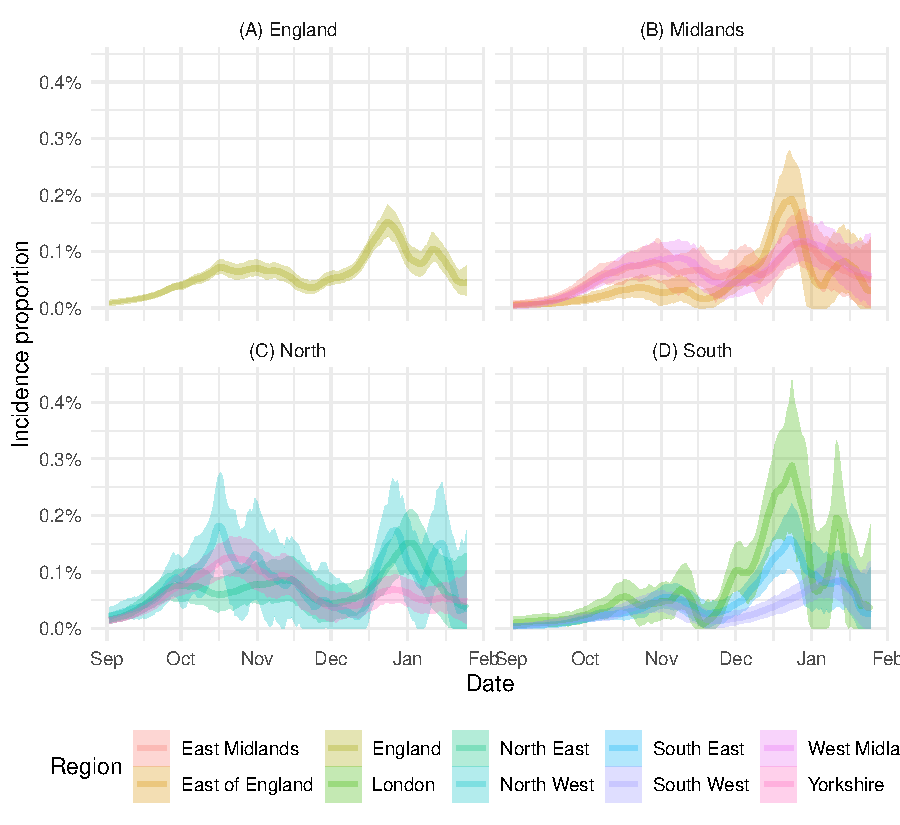
\includegraphics{transmission/backcalc-regions}
    \caption[Incidence estimated using backcalculation by region]{%
        Incidence proportion for all of England (A) and its component regions.
        Regions are split into broad groupings of three regions each: Northern (B), Midlands (C), and Southern (D).
        Yorkshire and the Humber is labelled as Yorkshire for brevity.
    }
    \label{transmission:fig:backcalc-regions}
\end{figure}

The incidence proportion was highest among the 11--15 and 16--25 age groups throughout the period (see \cref{transmission:fig:backcalc-ages}).
Except the 16--25 age group, all age groups show similar trends (\ie parallel lines on a log scale).
This is the pattern predicted by an age-stratified, mechanistic transmission model (such as the one introduced in \cref{E-SEIR:sec:structured-populations}), if behavioural changes are independent of age group, and there is negligible impact of immunity.
The incidence proportion in the 16--25 age group decreases faster than other age groups during November.
There are many plausible explanations for this effect.
The higher incidence in this age group prior to November means it could be an immunity effect.
Alternatively, it could be a consequence of schools remaining open in the November lockdown; 20--24 year olds rarely interact with school-aged children (see \cref{E-SEIR:fig:age-contacts})
Many other explanations are possible, and further work is required to determine causality.
\begin{figure}
    \makebox[\textwidth][c]{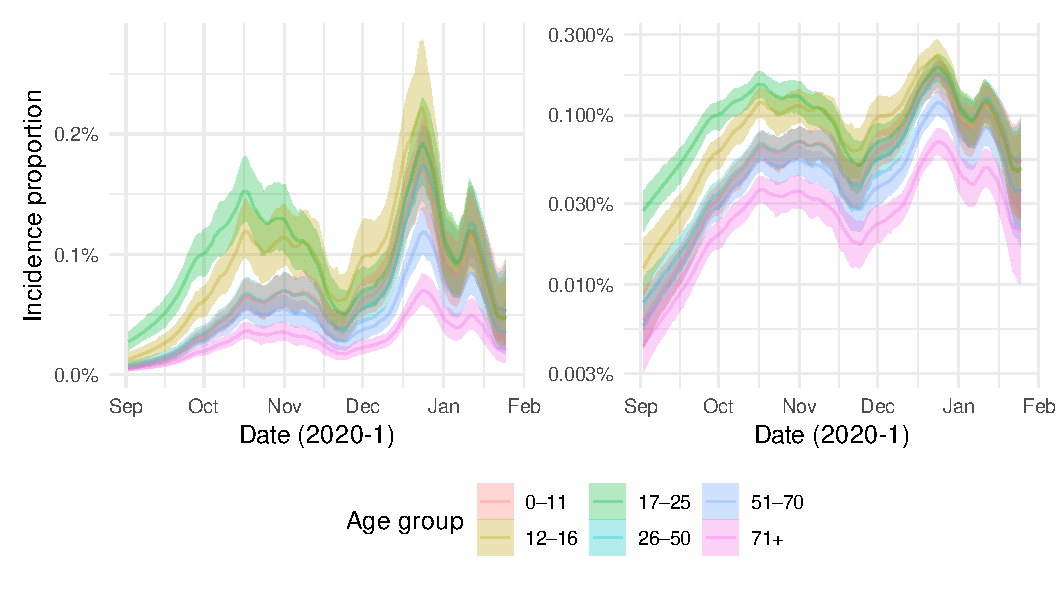
\includegraphics[width=.9\paperwidth]{transmission/backcalc-ages}}
    \caption[Incidence estimated using backcalculation by age group]{%
        Incidence proportion for each age group, on both natural and log scales.
    }
    \label{transmission:fig:backcalc-ages}
\end{figure}

An edge effect where a rapid rise is seen between day 1 and 2 is visible (see \cref{transmission:fig:backcalc-start-effect}).
This is due to the incorrect assumption that incidence is constant in the past.
Changing this assumption (\eg to exponential growth) modifies the estimated value on the first day, but the rest of the series is insensitive to this change (not shown).
Therefore, the first day's estimate is unreliable, and has been excluded from all other plots.
However, the rest of the series is robust to this assumption and hence reliable.
\begin{figure}
    \centering 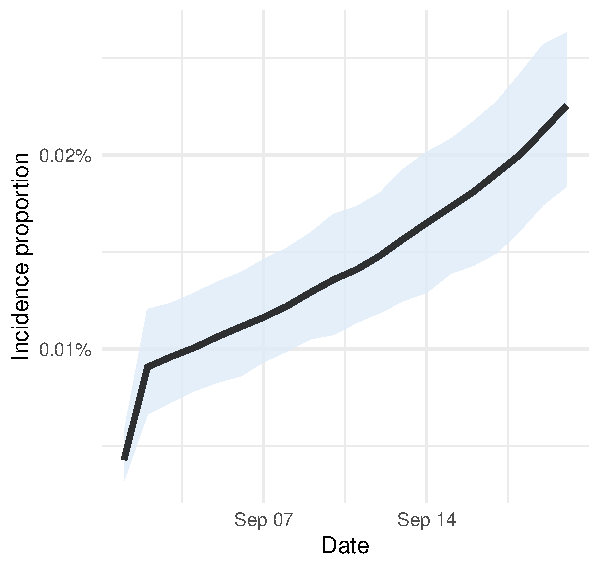
\includegraphics{transmission/backcalc-start-effect}
    \caption[Edge effects in backcalculation method]{%
        First seven days of incidence proportion estimate for the whole of England, highlighting the edge effect.
    }
    \label{transmission:fig:backcalc-start-effect}
\end{figure}

\section{Mechanistic modelling} \label{SEIR}

There are various advantages to using a mechanistic model to estimate transmission (see \cref{E-inc-prev:sec:infection-process}).
This section applies the mechanistic modelling framework introduced in \cref{E-SEIR:sec:mechanistic-models} to estimate the transmission of SARS-CoV-2 in England.

The transmission part of the model follows \textcite{birrellRealtime}.
A novel approach (\cref{SEIR:sec:observation}) links the transmission model to the data.
In the mechanistic modelling literature, this part of the model is referred to as the observation model; however, in the terminology of \cref{E-inc-prev}, it includes both the prevalence process and the observation process.

This section uses the same notation as \cref{E-SEIR:sec:mechanistic-models}, following the infectious disease modelling literature rather than the statistical conventions used elsewhere in this thesis.

\subsection{Methods}

% The model will be stratified only by region and age group, so the data are aggregated to these levels.
% Only individuals aged two or older are eligible to participate in the CIS; I assume that test results in all participants aged under 11 are still representative of the whole $[0, 11)$ age group.

I model each region fully independently, \ie with no shared parameters or transmission between regions.
As well as the motivation given in \cref{E-backcalc}, independent regions allows heterogeneity in the parameters between regions, which could arise from a range of socioeconomic factors.
Furthermore, the assumption of homogeneous mixing within age groups is more plausible for regions than the whole of England.
By modelling each region independently, I assume that the epidemics in each region do not interact.
Clearly, this is not realistic as travel between regions of England is common and unrestricted.
However, for a large epidemic, the non-interaction is a good approximation~\autocite{birrellRealtimea}.

\subsubsection{WAIFW matrix}

A parsimonious model is needed to parameterise the WAIFW matrix (see \cref{E-SEIR:sec:structured-populations}).
I follow the WAIFW matrix parameterisation of \textcite{birrellRealtime}, decomposing the rate of transmission from individuals in age group $a'$ to susceptible individuals in age group $a$ as $\beta_{aa'}(t) = \beta(t) \kappa_{aa'}(t) q_{aa'} N_{a'}$.
This separates contact patterns, $\kappa_{aa'}$, which can vary over time; transmission probability upon contact between age groups $a$ and $a'$, $q_{aa'}$, assumed constant; a region-wide effect for time, $\beta(t)$; and the population of the stratum, $N_{a'}$.

I take information on the contact rates, $\kappa_{aa'}(t)$, from several data sources, using the methodology of \textcite{vanleeuwenTime,vanleeuwenAugmenting}.
%; these estimates have been used for previous modelling of the COVID-19 pandemic~\autocite{vanleeuwenTime,birrellRealtime}.
% These start with estimates of contact in each setting, based on \textcite{vanleeuwenAugmenting}.
This method starts with pre-pandemic baseline estimates of: $\kappa_{aa'}$ from the POLYMOD study~\autocite{mossongSocial}, and time use from the UK Time Use Survey (UKTUS)~\autocite{UKTUS}.
POLYMOD asked a representative sample of the UK population about the contacts they make each day, including information on each contact's age and location (home, work, school, leisure, transport, or other).
UKTUS asked a representative sample of the UK population about how much time they spent doing various activities (\eg shopping and spending time at home) each day.
\Textcite{vanleeuwenAugmenting} combined these two datasets to estimate the rate of contacts between age groups during each activity.
\Textcite{birrellRealtime} then modify these contact rates based on measured changes in time use during the pandemic.
These changes are measured using Google mobility data~\autocite{googleCOVID19} and school attendance data~(unpublished).
Google mobility data is based on the location of Android users over time, relative to a pre-pandemic baseline.
The mobility and school data are averaged over a week then used to down or up-weight the number of contacts in each setting, before combining contacts across settings to form $\kappa_{aa'}(t)$.
$\kappa_{aa'}(t)$ is assumed to be piecewise constant, changing only at the start of each week.
For further details see \textcite{vanleeuwenAugmenting} and \textcite[supplementary material]{birrellRealtime}.

Some behavioural changes (\eg mask wearing) impact transmission.
However, these are not captured by the contact survey.
To allow for these changes and the uncertainty produced in formulating $\matr{\kappa}(t)$, I follow \textcite{birrellRealtime} in placing a random walk prior on $\log\beta(t)$  on the weekly timescale:
\begin{align}
    \beta(t) &= \beta_{\tilde{w}(t)} \\
    \log\beta_{w+1} &= \log\beta_w + \sigma_\epsilon \epsilon_w \\
    \epsilon_w &\sim \N(0, 1)
\end{align}
where $\tilde{w}(t)$ is the week number of time $t$, with week 1 being the first week considered.
Two hyperparameters will be inferred: $\beta_1$, the initial value of the random walk; and $\sigma_\epsilon$, the standard deviation of the random walk (see \cref{SEIR:sec:priors}).

% $K_{ij}$ and $\beta_{ij}$ appear only as a product and therefore are not individually identifiable.
% Normally, $K_{ij}$ is assumed to be known, for example from a previous contact survey~\autocite[such as][]{mossongSocial}.
% Ideally, all the $\beta_{ij}$ terms would be estimated, but there is normally inadequate data to do so, requiring assumptions to be made to reduce the number of parameters~\autocite[65]{keelingModeling}.
% % $\beta_{ij}$ is then estimated, although often with a parsimonious model
% A common assumption is that $\beta_{ij}$ can be decomposed into two independent components such that $\beta_{ij} = \beta \beta^\text{susc}_{i} \beta^\text{inf}_j$.
% For any stratum $i$, $\beta^\text{susc}_i$ is known as the \emph{relative susceptibility} of stratum $i$.

Finally, $q_{aa'}$ needs to be specified.
I follow a common approach\todo{cite anderson and may}, decomposing it into two independent factors such that $q_{aa'} = q^\text{susc}_{a} q^\text{inf}_{a'}$, where $q^\text{susc}_a$ is the \emph{susceptibility} of stratum $a$, \ie how vulnerable to infection individuals in stratum $a$ are; and $q^\text{inf}_{a'}$ is the \emph{transmissibility} of stratum $a'$, \ie how likely individuals in stratum $a$ are to pass on an infection.
% Then $\beta^\text{susc}_i$ is the relative risk of an individual in stratum $i$ being infected, relative to an individual in stratum $a_0$.
These measures include both biological differences, \eg due to differences in immune systems, or behavioural, \eg if infants are less hygienic than adults.

%Now, we assume that $\beta_{ij} = \beta(t) \beta_{ij}$ where $\beta(t)$ is a non-strata-specific, time-varying component representing precautions taken by the population, for example masking; and $\beta_{ij}$ represents a constant probability of transmission from an infectious individual in strata $j$ to a susceptible individual in strata $i$ given contact, which could, for instance, be affected by differential susceptibility to infection for different age-groups.
%We arbitrarily choose one $\beta_{ij}$ to be equal to 1 for identifiability and hence the other $\beta_{ij}$ values are relative to this reference class.

Studies of pre-Alpha SARS-CoV-2 suggest that all individuals have similar infectiousness but that pre-adolescent children are less susceptible than adults~\autocite{chenRole,vinerTransmission}.
Therefore, I set $q^\text{inf}_{a'} = 1$ for all $a'$, $q^\text{susc}_{a} = q_c$ for 0--11 year olds, and $q^\text{susc}_{a} = 1$ for the remaining strata.
$q_c$ can be interpreted as the relative probability that a child is infected (compared to an adult), given contact with an infectious individual.
$q_c$ is then estimated, although using an informative prior (see \cref{SEIR:sec:priors}).

\subsubsection{Prevalence and observation models} \label{SEIR:sec:observation}

\todo[inline]{consider if this paragraph is too repetitive}

The transmission model represents the infection process (introduced in \cref{E-inc-prev:sec:infection-process}).
A variety of different approaches can be taken to link a transmission model to observations.
In the context of CIS, this requires representing the prevalence and observation processes (introduced in \cref{E-inc-prev:sec:prevalence-process,E-inc-prev:sec:observation-process} respectively).
The method to do so is known as the observation model.
The formulation of this model is heavily dependent on the data available.
This means that there is a wide variety of models used.
This section  explains the novel modelling approach I propose for fitting to the CIS prevalence data.

% Here, I extend the system of ODEs to include compartments representing RT-PCR positive individuals.
% The proportion of RT-PCR positive individuals in each strata is then linked to the CIS using a Beta-Binomial likelihood, with the modelled proportion that are RT-PCR positive as the mean of the Beta distribution.
One approach would be to convolve the incidence based on the transmission model with the RT-PCR duration distribution.
Here, the daily incidence proportion for each stratum is by solving the system of ODEs governing the transmission model, and then prevalence calculated as using \cref{E-inc-prev:eq:EPt}.
However, this approach is computationally expensive, likely prohibitively so if performed within a MCMC loop.

A computationally cheaper option, which I will take, is to approximate this convolution by adding compartments to the ODEs.
This approach allows a infected, pre-positive compartment, which I denote $p_0$, to be included simply.
$p_0$ increases at the same rate as individuals flow into $e_1$.
These individuals then transition into a set of compartment with their transition rates, $p_1, \dots, p_l$, chosen to match the duration of positivity estimates in \cref{E-imperf-test}.
These compartments do not have a biological interpretation; the same idea is behind having multiple exposed or latent compartments (introduced in \cref{E-SEIR:sec:non-exponential}).

Deciding $l$ and the length of time each individual spends in each compartment is the most challenging part of formulating the observation model.
The class of distributions which can be represented as a series of compartments are known as \emph{phase-type} distributions.
Discussions of general phase-type distributions are beyond the scope of this thesis; a review in a biological context can be found in \textcite{hobolthPhasetype}.
I will restrict myself to the subset of phase-type distributions defined by \textcite{osogamiClosed} as Erlang-Coxian (EC) distributions.
EC distributions are convenient because they are flexible enough to approximate almost any distribution, and the parameters of the approximation are given by closed-form functions of the distribution's moments.

% Formally, a phase-type distribution as the distribution of \emph{absorption time} in a \emph{continuous-time Markov process} with a single absorbing state~\autocite{hobolthPhasetype}.
% Given a probability distribution over starting states, a rate at which 
% The process can be defined by its size, $l$, a $l \times l$ \emph{transition matrix}, $\matr{M} \in \reals^{l \times l}$, an \emph{exit rate} vector, $\vec{\alpha}$ 
% The process's state at time $t$, $W_t$, is a scalar $W_t \in \{ 1, \dots, l+1 \}$.
% Its transition matrix is defined, for $j \neq k$, as $\prob(W_{t+\delta t} = k \mid ) = M_{jk} \delta t$ for small, positive $\delta t$.
% The diagonal is defined as $M_{jj} = - \sum_{k \neq j} M_{jk}$ so that the matrix $\matr{M}$ has row sums 0.
% The state $l+1$ is an absorbing state, that is $\prob(W_{t+t'} = l+1 \mid W_t = l_1) = 1$ for any non-negative $t'$ (once the process enters it, it cannot leave).
% The exit rate gives the transition rates into the absorbing state: $\prob(W_{t+\delta t} = l + 1 \mid W_t = j) = \alpha_j \delta t$ for small $\delta t$.
% The process's absorption time is when it first arrives at the absorbing state, $\tau = \inf \{ t \ssep W_t = l+1 \}$.
% That is, $P$ is a phase-type distribution if it can be represented as a process 
% They are additions of arbitrary exponential distributions, and can (if there is no limit on the number of compartments used) represent any distribution.
% \todo{check/cite these claims}
% I use the method of \textcite{osogamiClosed} to determine $l$ and the transition rates between the compartments.

% A $l$-phase EC distribution is the sum of a $(l-2)$-phase gamma distribution and a two-phase acyclic, arbitrary phase-type distribution.
An EC distribution $P$ can be defined as the sum of three random variables: $K$, $X_1$, and $X_2$.
It is shown schematically in \cref{SEIR:fig:EC}.
Here, $K \dist \GamDist(l-2, \omega_Y)$, $X_1 \dist \Exponential(\omega_{X1})$ and $X_2$ is a mixture distribution taking the value 0 with probability $1-p_x$ or otherwise (\ie with probability $p_x$) distributed $\Exponential(\omega_{X2})$.
% The time between entering the 1st state and the $l+1$th state, the absorbing state, is the duration.
These distributions contain five parameters.
Three are positive reals, $\omega_Y$, $\omega_{X1}$, and $\omega_{X2}$; one is a probability, $p_x$, in the interval $[0, 1]$; and one is a positive integer, $l$.

The name Erlang-Coxian comes from the two distributions that make up the EC distribution.
Gamma distributions with integer first parameters (as $K$ has) are also known as Erlang distributions.
The distribution $X_1 + X_2$ is a special case of the Coxian distribution.
Hence, the overall distribution is known as a Erlang-Coxian distribution.

\begin{figure}
\makebox[\textwidth][c]{
\begin{tikzpicture}[
    node distance = 2.5cm,
    on grid,
    auto,
    ->,>=stealth',
    every state/.style={draw,rectangle},
    ]

    \node[state] (1) {1};
    \node[state, right of=1] (2) {2};
    \node[state, right of=2, draw=none] (dots) {$\dots$};
    \node[state, right of=dots] (lm2) {$l-2$};
    \node[state, right of=lm2] (lm1) {$l-1$};
    \node[state, right of=lm1] (l) {$l$};
    \node[state, right of=l, align=center] (absorbing) {absorbing\\state};

    \path (1) edge node {$\omega_Y$} (2)
          (2) edge node {$\omega_Y$} (dots)
          (dots) edge node {$\omega_Y$} (lm2)
          (lm2) edge node {$\omega_Y$} (lm1)
          (lm1) edge node {$p_x \omega_{X1}$} (l)
                edge [out=-45,in=-135] node[below] {$(1 - p_x) \omega_{X1}$} (absorbing)
          (l) edge node {$\omega_{X2}$} (absorbing);
\end{tikzpicture}
}
\caption[A $l$ phase EC distribution.]{Representation of an EC distribution as a series of compartments. The distribution is the time from entering state 1 and entering the absorbing state. The time between entering state 1 and state $l-2$ is distributed $K \dist \GamDist(l-2, \omega_Y)$, also known as an Erlang distribution. The time between entering state $l-2$ and the absorbing state has a Coxian distribution (see the main text for details).}
\label{SEIR:fig:EC}
\end{figure}

\Textcite{osogamiClosed} define a phase-type distribution $P$ as well representing an arbitrary distribution $G$ if $P$ and $G$ have the same first three moments.
They then prove that EC distributions have the following properties.
\begin{itemize}
    \item Let $\set{W}$ be the set of all phase-types distributions that well represent $G$ and $w$ be the minimum number of phases of any member of $\set{W}$. If $\set{W}$ is non-empty, then there exists a $l$-phase EC distribution $P' \in \set{W}$.
    \item Furthermore, at least one such $P'$ has $l \leq w + 1$. Fewer phases is generally beneficial as it reduces the time and space complexity of working with the distribution.
    \item The parameters of a $P'$ with $l \leq w + 1$ can be found using a closed-form expression (given by \textcite{osogamiClosed}). This is beneficial because finding arbitrary members of $\set{W}$ is a hard problem.
\end{itemize}

A total of five parameters are required to specify a $l$-phase EC distribution.
\begin{itemize}
    \item $l$, the number of phases.
    \item $\omega_Y$, the rate parameter of the Erlang distribution.
    \item $\omega_{X1}$, the rate parameter of the first state after the Erlang distribution.
    \item $\omega_{X2}$, the rate parameter of the second state after the Erlang distribution.
    \item $p_x$, the probability of moving from the end state of the Erlang distribution to the second (as opposed to directly to the absorbing state).
\end{itemize}

The mapfit package~\autocite{mapfit} implements the expressions to calculate the EC distribution parameters given a distribution's first three moments.
Applying the package to the posterior mean of the distribution estimated in \cref{E-imperf-test} gives the parameter estimates in \cref{SEIR:table:ec-params}.
\begin{table}
    \centering
    \begin{tabular}{c c c c c}
        $l$ & $\omega_Y$ & $\omega_{X1}$ & $\omega_{X2}$ & $p_x$ \\
        3 & 0.0820 & 0.126 & 0.0223 & 0.00973  \\
    \end{tabular}
    \caption{Parameter estimates for the EC distribution approximating the posterior mean of the duration distribution estimated in \cref{E-imperf-test}.}
    \label{SEIR:table:ec-params}
\end{table}
% end table of ec params

I link the modelled proportion of individuals that are RT-PCR positive to the data using a beta-binomial likelihood (as discussed in \cref{transmission:sec:data}).
If on each day $t$, each strata $i$ is observed to have $y_{it}$ positives out of $n_{it}$ tests, then the likelihood is:
\begin{align}
    \prod_{a,t} \BB (y_{at} \mid n_{at}, \sum_{k=1}^l \bar{p}_{kat}, \rho)
    \label{SEIR:eq:likelihood}
\end{align}
where $\bar{p}_{kat} = \int_{t}^{t+1} p_{ka}(s) ds$ is the mean occupancy in compartment $p_k$ and strata $a$ over day $t$ and $\rho$ is a nuisance parameter controlling the overdispersion of the beta-binomial distribution.

\subsubsection{Model equations and solution} \label{SEIR:sec:full-model}

\begin{figure}
\makebox[\textwidth][c]{
\begin{tikzpicture}[
    node distance = 2.5cm,
    on grid,
    auto,
    ->,>=stealth',
    every state/.style={draw,rectangle},
    ]

    \node[state] (S) {$s$};
    \node[state, right=of S] (E1) {$e_1$};
    \node[state, right=of E1] (E2) {$e_2$};
    \node[state, right=of E2] (I1) {$i_1$};
    \node[state, right=of I1] (I2) {$i_2$};
    \node[state, right=of I2] (R) {$r$};

    \path (S) edge node {$\lambda$} (E1)
          (E1) edge node {$\sigma$} (E2)
          (E2) edge node {$\sigma$} (I1)
          (I1) edge node {$\gamma$} (I2)
          (I2) edge node {$\gamma$} (R);

    \node[state, below=3cm of E1] (P0) {$p_0$};
    \node[state, right=of P0] (P1) {$p_1$};
    \node[state, right=of P1] (P2) {$p_2$};
    \node[state, right=of P2] (P3) {$p_3$};
    \node[state, right=of P3, draw=none] (P4) {};

    \path  (S) edge node {$\lambda$} (P0)
          (P0) edge node {$\omega_0$} (P1)
          (P1) edge node {$\omega_Y$} (P2)
          (P2) edge node {$p_x \omega_{X1}$} (P3)
               edge [out=-45,in=-135] node[below] {$(1 - p_x) \omega_{X1}$} (P4)
          (P3) edge node {$\omega_{X2}$} (P4);
    
    \node[draw, thick, inner sep=0.3cm, fit=(P1) (P3), fill=blue!10,opacity=0.2] {};
\end{tikzpicture}
}
  \caption[SEIR model]{SEIR model used for the analysis in this section. The shaded box represents RT-PCR-positive individuals. Shown for a single stratum.}
  \label{SEIR:fig:full-model}
\end{figure}

The remaining details of the transmission model structure follow \textcite{birrellRealtime}.
The transmission model is a SEIR model with two latent and two infectious states.
To form whole of England estimates, each region is modelled independently with the results aggregated, using the poststratification methodology explained in \cref{E-backcalc}.

A diagram of the model for a single stratum is shown in figure \cref{SEIR:fig:full-model}.
The full system of differential equations for each region is below.
\begin{align}
    \label{SEIR:eq:fullODEs}
    \vec{\lambda}(t) &= \beta(t) (\matr{\kappa}(t) \circ \matr{q}) (\vec{i_1}(t) + \vec{i_2}(t)) \\
    \frac{d\vec{s}(t)}{dt} &= -\vec{\lambda}(t) \circ \vec{s}(t) \\
    \frac{d\vec{e_1}(t)}{dt} &= \vec{\lambda}(t) \circ \vec{s}(t) - 2\sigma \vec{e_1}(t) \\
    \frac{d\vec{e_2}(t)}{dt} &= 2\sigma \vec{e_1}(t) - 2\sigma \vec{e_2}(t) \\
    \frac{d\vec{i_1}(t)}{dt} &= 2\sigma \vec{e_2}(t) - 2\gamma \vec{i_1}(t) \\
    \frac{d\vec{i_2}(t)}{dt} &= 2\gamma \vec{i_1}(t) - 2\gamma \vec{i_2}(t) \\
    \frac{d\vec{r}(t)}{dt} &= 2\gamma \vec{i_2}(t) \\
    \frac{d\vec{p_0}(t)}{dt} &= \vec{\lambda} \circ \vec{s}(t) - \omega_0 \vec{p_0}(t) \\
    \frac{d\vec{p_1}(t)}{dt} &= \omega_0 \vec{p_0}(t) - \omega_Y \vec{p_1}(t) \\
    \frac{d\vec{p_2}(t)}{dt} &= \omega_Y \vec{p_1}(t) - \omega_{X1} \vec{p_2}(t) \\
    \frac{d\vec{p_3}(t)}{dt} &= p_x \omega_{X1} \vec{p_2}(t) - \omega_{X2} \vec{p_3}(t).
\end{align}

I solve the system of ODEs using Euler's method, discretised at timesteps of $\delta t = 1/2$ days.
That is, if $\vec{x}_t$ is the system state at time $t$ for $t \in \{ 0, 0.5, 1, \dots \}$ then $x_{t+\frac{1}{2}} = x_t + (d\vec{x}(t)/dt) \delta t$

The mean prevalence on day $t$, used for the likelihood (see \cref{SEIR:eq:likelihood}), can be calculated as $\bar{p}_{kat} = \frac{1}{2} ( p_{kat} + p_{ka,t+1/2} )$.

\subsubsection{Priors} \label{SEIR:sec:priors}

Priors for the parameters are given in \cref{SEIR:table:priors}.
The parameters governing the duration of positivity ($\omega$s) were explained previously (see \cref{SEIR:table:ec-params}).
The initial conditions and transition rate parameters are unindentifiable in a SEIR model~\autocite{dankwaStructural}, therefore strongly informative priors are used for them.
$\sigma_\epsilon$ and $\rho$ are given priors that penalise model complexity.
The prior on $\sigma_\epsilon$ is a penalised complexity prior, favouring a null model of constant values for $\beta(t)$~\autocite{simpsonPenalising}.
The prior on $\rho$ favours a null model of a binomial likelihood.
The remaining parameters have weakly informative priors.

\begin{landscape}
\begin{table}
\begin{tabular}{l c l l}
    Parameter description & Symbol & Distribution & Comment \\
    \hline \\
    Mean latent period & $1/\sigma$ & 3.5 days (fixed) & Based on \textcite{zhaoEstimating} \\
    Mean infectious period & $1/\gamma$ & 4 days (fixed) & Based on \textcite{zhaoEstimating} \\
    Initial proportion without immunity & $\vec\pi$ & See \cref{SEIR:table:immunity-prior} & \\
    Initial proportion infectious & $i^+$ & $\BetaDist(0.5, 1000)$ & Weakly informative \\
    Susceptibility of children & $q_c$ & $\LN(-0.4325, 0.1174)$ & Based on \textcite{vinerTransmission}  \\
    Initial growth rate & $\psi$ & $\N(0.06, 0.04)$ & Weakly informative \\
    Standard deviation of random walk steps on log scale & $\sigma_\epsilon$ & $\Exponential(80)$ & Penalising towards constant \\
    Overdispersion of observations & $\rho$ & $\Exponential(2 \times 10^5)$ & Penalising towards binomial
\end{tabular}
\caption[SEIR model priors]{Priors for each parameter. For details of the distributions and their parameterisations see \cref{E-distributions}.}
\label{SEIR:table:priors}
\end{table}

\begin{table}
\centering
\begin{tabular}{l|lllll}
         & $[0,16)$ & $[16,25)$ & $[25,50)$ & $[50,70)$ & $[70,\infty)$ \\
        \hline
        East Midlands & $\BetaDist(8.5, 301)$ & $\BetaDist(18, 256)$ & $\BetaDist(19, 475)$ & $\BetaDist(20, 493)$ & $\BetaDist(5, 337)$ \\
        East of England & $\BetaDist(7.9, 236)$ & $\BetaDist(21, 248)$ & $\BetaDist(35, 677)$ & $\BetaDist(26, 613)$ & $\BetaDist(5.6, 332)$ \\
        London & $\BetaDist(9.7, 131)$ & $\BetaDist(50, 328)$ & $\BetaDist(154, 1331)$ & $\BetaDist(106, 990)$ & $\BetaDist(7.6, 204)$ \\
        North East & $\BetaDist(6.1, 180)$ & $\BetaDist(12, 145)$ & $\BetaDist(14, 274)$ & $\BetaDist(14, 295)$ & $\BetaDist(4.2, 240)$ \\
        North West & $\BetaDist(12, 252)$ & $\BetaDist(38, 353)$ & $\BetaDist(72, 885)$ & $\BetaDist(44, 695)$ & $\BetaDist(6.3, 264)$ \\
        South East & $\BetaDist(8.9, 404)$ & $\BetaDist(17, 319)$ & $\BetaDist(20, 577)$ & $\BetaDist(19, 586)$ & $\BetaDist(4.4, 356)$ \\
        South West & $\BetaDist(6.9, 415)$ & $\BetaDist(11, 277)$ & $\BetaDist(12, 556)$ & $\BetaDist(11, 559)$ & $\BetaDist(4, 492)$ \\
        West Midlands & $\BetaDist(8, 167)$ & $\BetaDist(19, 151)$ & $\BetaDist(32, 475)$ & $\BetaDist(33, 504)$ & $\BetaDist(5.8, 241)$ \\
        Yorkshire and The Humber & $\BetaDist(9.2, 314)$ & $\BetaDist(19, 242)$ & $\BetaDist(27, 589)$ & $\BetaDist(18, 474)$ & $\BetaDist(4.9, 316)$ \\
    \end{tabular}
\caption{Priors for $\vec{\pi}$, the proportion of the population without prior immunity, in each age group and region combination. Based on seroprevalence in blood donors~\autocite{amirthalingamSeroprevalence} and a representative sample of children~\autocite{ratcliffeCommunity} in August 2020.}
\label{SEIR:table:immunity-prior}
\end{table}
\end{landscape}

\subsubsection{Inference} \label{SEIR:sec:inference}

I compute the posterior distribution using MCMC.
Specifically, I use an adaptive random-walk Metropolis-Hastings algorithm (previously discussed in \cref{E-inc-prev:sec:MCMC}).
The proposal distribution is a multivariate normal that adapts to the covariance of the posterior.
The adaption algorithm is based on \textcite[algorithm 4]{andrieuTutorial}, with the implementation based on \textcite{ghoshApproximate}'s work.
Proposals are accepted or rejected using the standard Metropolis-Hastings (MH) acceptance probability.
See \cref{SEIR:MCMC-algorithm} for full details.
\begin{algorithm}
 set $\vec{X_0}$ to an initial value of the parameter vector \;
 $\vec{\mu_0} = \vec{X_0}$ \;
 $\matr{\Sigma_0} = \text{diag}(\vec{\mu_0})$ \;
 $\lambda_0 = 1$ \;
 \For{$i = 1, \dots, M$}{
  sample $\vec{Y_}i \sim \N(\vec{\mu_{i-1}}, \lambda_{i-1}\matr{\Sigma_{i-1}})$\;
  set $\vec{X_i}$ to $\vec{Y_i}$ or $\vec{X_{i-1}}$ using a MH acceptance step\;
  update the proportion of proposals accepted so far, $\alpha$ \;
  \eIf(\tcc{No adaptation for 200 iterations}){$i \leq 200$}{
    $\lambda_i = \lambda_{i-1}$ \;
    $\vec{\mu_i} = \vec{\mu_{i-1}}$ \;
    $\matr{\Sigma_i} = \matr{\Sigma_{i-1}}$ \;
   }{
    $\gamma_i = (i - 200)^{-0.6}$ \;
    $\log \lambda_i = \log \lambda_{i-1} + \gamma_i(\alpha - 0.234)$ \;
    $\vec{\mu_i} = (1 - \gamma_i) \vec{\mu_{i-1}} + \gamma_i \vec{X_i}$ \;
    $\matr{\Sigma_i} = (1 - \gamma_i) \matr{\Sigma_{i-1}} + \gamma_i (\vec{X_i} - \vec{\mu_i})(\vec{X_i} - \vec{\mu_i})^T$ \;
  }
 }
 \caption{Algorithm for adaptive random-walk Metropolis-Hastings. $\vec{\mu_i}$ and $\matr{\Sigma_i}$ are an estimate of the mean and covariance of the posterior distribution using information up to iteration $i$. $\text{diag}(\vec{\mu_0})$ is the diagonal matrix with diagonal entries equal to $\vec{\mu_0}$. $\lambda_i$ is the scale parameter of the proposal distribution at iteration $i$, tuned to try and ensure an optimal proportion of proposals are accepted (23.4\%). $\gamma_i$ is the learning rate, which determines how much adaptation occurs. $\gamma_i \to 0$ as $i \to \infty$ so the rate of adaptation is \emph{vanishing}. Vanishing adaptation is required for the algorithm to converge to the target distribution~\autocite[section 3]{andrieuTutorial}.}
 \label{SEIR:MCMC-algorithm}
\end{algorithm}

I transformed parameters with restricted ranges for sampling, to improve efficiency.
Parameters which are constrained to the positive reals ($\sigma_\epsilon$, $\rho$, and $q_c$) were sampled on the log scale.
Parameters which are constrained to the unit interval ($i^+$ and $\vec{\pi}$) were sampled on the logit scale.

I run 4 chains for 1,000,000 iterations each.
The first 500,000 were discarded as burn-in, with the remaining chains thinned to every 100th iteration.
This gives 5,000 posterior samples per region.
This was further thinned to 2,000 samples when calculating posterior predictive quantities (incidence and prevalence) due to their computational cost.

Following \textcite{birrellBayesian}, I reparameterise the model to improve identifiability.
Rather than directly inferring $\beta_1$, I infer the initial growth rate of the epidemic.
In addition, I use a parsimonious parameterisation of the initial conditions using the initial proportion of the population that are infectious and the initial proportion that are susceptible only.
Both of these rely on an assumption that the epidemic is in a steady-state exponential growth phase at time 0 (see \cref{E-SEIR:sec:SIR}).

During such an exponential growth phase, all components of the $\vec{e}$, $\vec{i}$ and $\vec{p}$ compartments grow at the same growth rate, $\psi$.
This follows directly from the ODEs if $\vec{s}$ is constant. 
The growth rate $\psi$ is easily identifiable from the data, and therefore a parameterisation in terms of $\phi$ should be more computationally efficient.
If this is the initial exponential phase, when $\vec{s} \approx 1$, then the basic reproduction number for a SEIR model is linked to this growth rate by~\autocite{birrellBayesian,wearingAppropriate}:
\begin{align}
    \R = \frac{\psi \left( \frac{\psi}{2\sigma} + 1 \right)^2}{\gamma \left(1 - \frac{1}{\left(\frac{\psi}{2 \gamma} + 1 \right)^2} \right)} \label{SEIR:eq:rtoR}.
\end{align}

$\R$ can also be expressed a function of $\matr{\beta}(0)$, and hence $\beta_1$ (as explained in \cref{E-SEIR:sec:structured-populations}).
Combining these expressions, the model can be parameterised by using $\psi$ in place of $\beta_1$ by using the following procedure.
Start by calculating $\R$ from $\psi$ using \cref{SEIR:eq:rtoR}; denote this $\hat{R}$.
$\hat{R}$ is the $\R$ that the current value of $\psi$ implies.
Hence, $\beta_1$ should be set such that $\matr{\beta}(0)$ implies $\R = \hat{R}$.
To do so, define $R^*$ as $\R$ $\beta_1 = 1$.
Using the results of \cref{E-SEIR:sec:structured-populations}, $R^* = D(\matr{\beta}(0)) / \gamma$, computed using $\beta_1=1$ (recall that $D(\matr{\beta})$ denotes the dominant eigenvalue of $\matr{\beta}$).
Finally, set $\beta_1 = \hat{R} / R^*$; as multiplying a matrix by a scalar also multiplies its dominant eigenvalue by that same scalar, this means that $\R$ at time 0 is $\hat{R}$, as desired.

To form a parsimonious parameterisation of the initial state, first focus on the initial proportion of the population that is in the infectious compartments.
Recall, from \cref{E-SEIR:sec:structured-populations}, that in the exponential growth phase, the relative proportion of each stratum that is infectious is proportional to the dominant eigenvector of $\matr{\beta}$, which I denote $\vec{d}$.
Introduce a model parameter $i^+$, the proportion of the population in the $i$ states at time 0 in the strata with the highest proportion infectious.
Define the total number of infectious individuals at time 0 as $\vec{i_0} = \vec{i_1} + \vec{i_2} = \frac{i^+}{\max \vec{d}} \vec{d}$.

From the system of ODEs, the knowledge that all the compartments are growing exponentially at rate $\psi$, and the parameters $\vec{\pi}$ (where $\pi_a$ is the proportion of strata $i$ without immunity at time 0, hence, $\vec{r} = 1 - \vec{\pi}$) one can derive the following for the initial state of the compartments:
\begin{align}
    \vec{i_1} &= \vec{i_0} \left(1 + \frac{2\gamma}{\psi + 2\gamma} \right)^{-1} \\
    \vec{i_2} &= \vec{i_0} - \vec{i_1} \\
    \vec{e_2} &= \vec{i_1} \frac{\psi + 2\gamma}{2\sigma} \\
    \vec{e_1} &= \vec{e_2} \frac{\psi + 2\sigma}{2\sigma} \\
    \vec{s} &= \vec{\pi} - \vec{i_0} - \vec{e_1} - \vec{e_2} \\
    \vec{p_0} &= \vec{e_1} \frac{\psi + 2\sigma}{\psi + \omega_0} \\
    \vec{p_1} &= \vec{p_0} \frac{\omega_0}{\psi + \omega_Y} \\
    \vec{p_2} &= \vec{p_1} \frac{\omega_Y}{\psi + \omega_{X1}} \\
    \vec{p_3} &= \vec{p_2} \frac{p_x \omega_{X1}}{\psi + \omega_{X2}}.
\end{align}

\subsection{Simulation study} \label{SEIR:sec:sim-study}

I ran a simulation study to check that the inference procedure (\cref{SEIR:sec:inference}) was working correctly and that the model was identifiable.
I ran 100 simulations, with parameters drawn from the priors (see \cref{SEIR:table:priors}) except that the prior on $\psi$ was $\LN(0.048, 0.0035)$.
I used the more informative prior for the simulation study to ensure that the simulations were realistic.
The weakly informative prior, used for the main analysis, allows a wide range of epidemics including some that are shrinking at the start of the time period.
Priors and population sizes were matched to the East of England region, over the same time period as the main analysis.

All other aspects of the simulation model, including $\matr{\kappa}$, are as previously described in this section.
This means that the simulations created realistic incidence and prevalence curves (see \cref{SEIR:fig:sim-data}).
In particular, the October half-term school holiday is visible, especially in the school-age groups and the November lockdown is visible to some extent in all age groups.
\begin{figure}
    \thisfloatpagestyle{empty}
    \vspace{-3cm}
    \makebox[\textwidth][c]{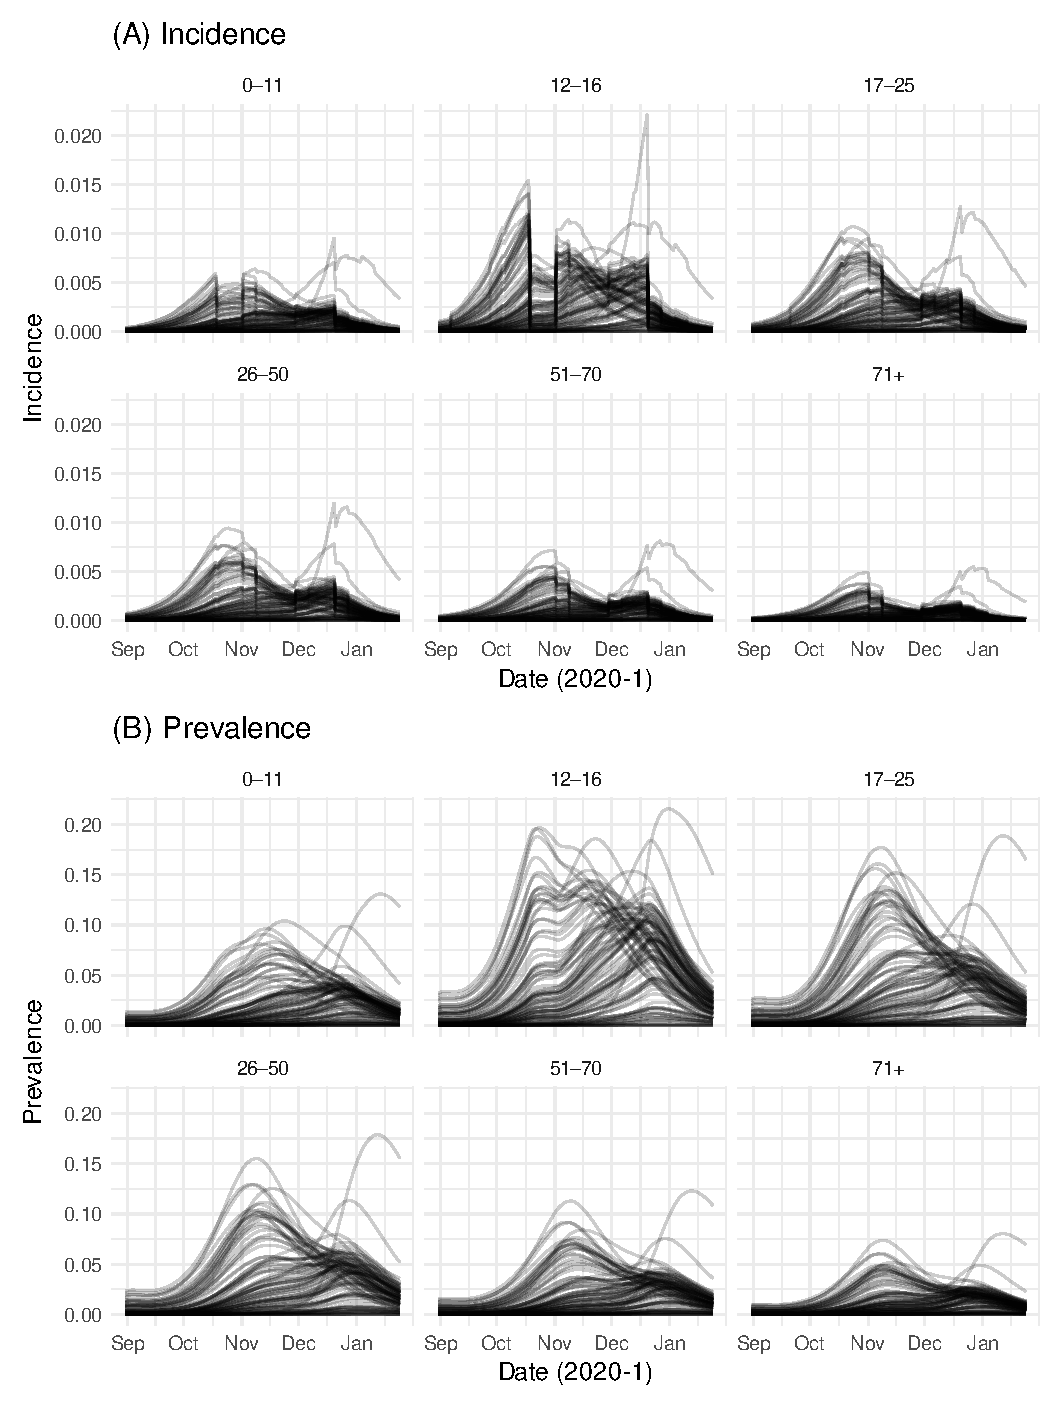
\includegraphics[width=.9\paperwidth]{SEIR/sim/data}}
    \caption[Simulated data]{%
        Incidence (top) and prevalence (bottom) for the 100 simulated data sets as a proportion of each stratum.
        Prevalence shown is $\bar{p}_{kat}$, the true population prevalence on each day, excluding sampling noise.
        Each line represents one simulation.
    }
    \label{SEIR:fig:sim-data}
\end{figure}

% Furthermore, the combination of the posteriors across all simulations should recover the prior.

To check the performance of the inference procedure, I calculated the coverage of the 50\%, 75\%, and 95\% central credible intervals for each parameter and simulation.
Define coverage as the proportion of simulations where the true value of the parameter in that simulation was within the credible interval.
As the parameters are drawn from the prior, if the inference is performed correctly then the coverage for each parameter should equal the nominal probability (\eg the coverage should be 50\% for the 50\% credible intervals)~\autocite{cookValidation}.
This check is related to, although simpler than, simulation-based calibration~\autocite{taltsValidating}.
I constructed a confidence interval for the coverage using the Pearson-Klopper method implemented in the binom package~\autocite{binom1-1}.

The majority of the confidence intervals contain the nominal probability (see \cref{SEIR:fig:sim-coverage}).
There is a tendency for the coverage to be slightly lower than the nominal probability, suggesting that the credible intervals are slightly too narrow.
This is a common issue with random walk MCMC (see \cref{E-inc-prev:sec:MCMC}).
This is similar when considering coverage of the derived quantities incidence and prevalence (see \cref{SEIR:fig:sim-inc-prev}).
\begin{figure}
    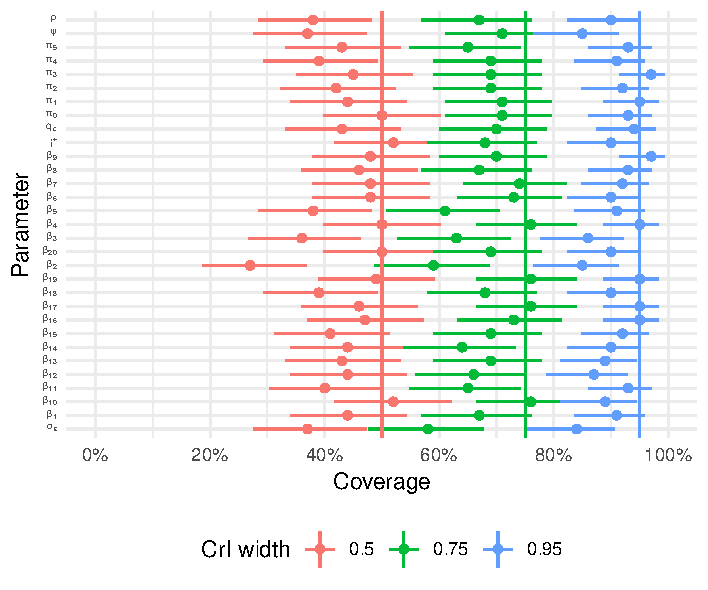
\includegraphics{SEIR/sim/coverage}
    \caption[Coverage of simulation study]{%
        Point estimate and 95\% confidence interval for coverage of the 50\%, 75\%, and 95\% central credible intervals for each parameter; see text for full definition.
        Vertical lines show the nominal coverage.
    }
    \label{SEIR:fig:sim-coverage}
\end{figure}
\begin{figure}
    \thisfloatpagestyle{empty}
    \vspace{-3cm}
    \makebox[\textwidth][c]{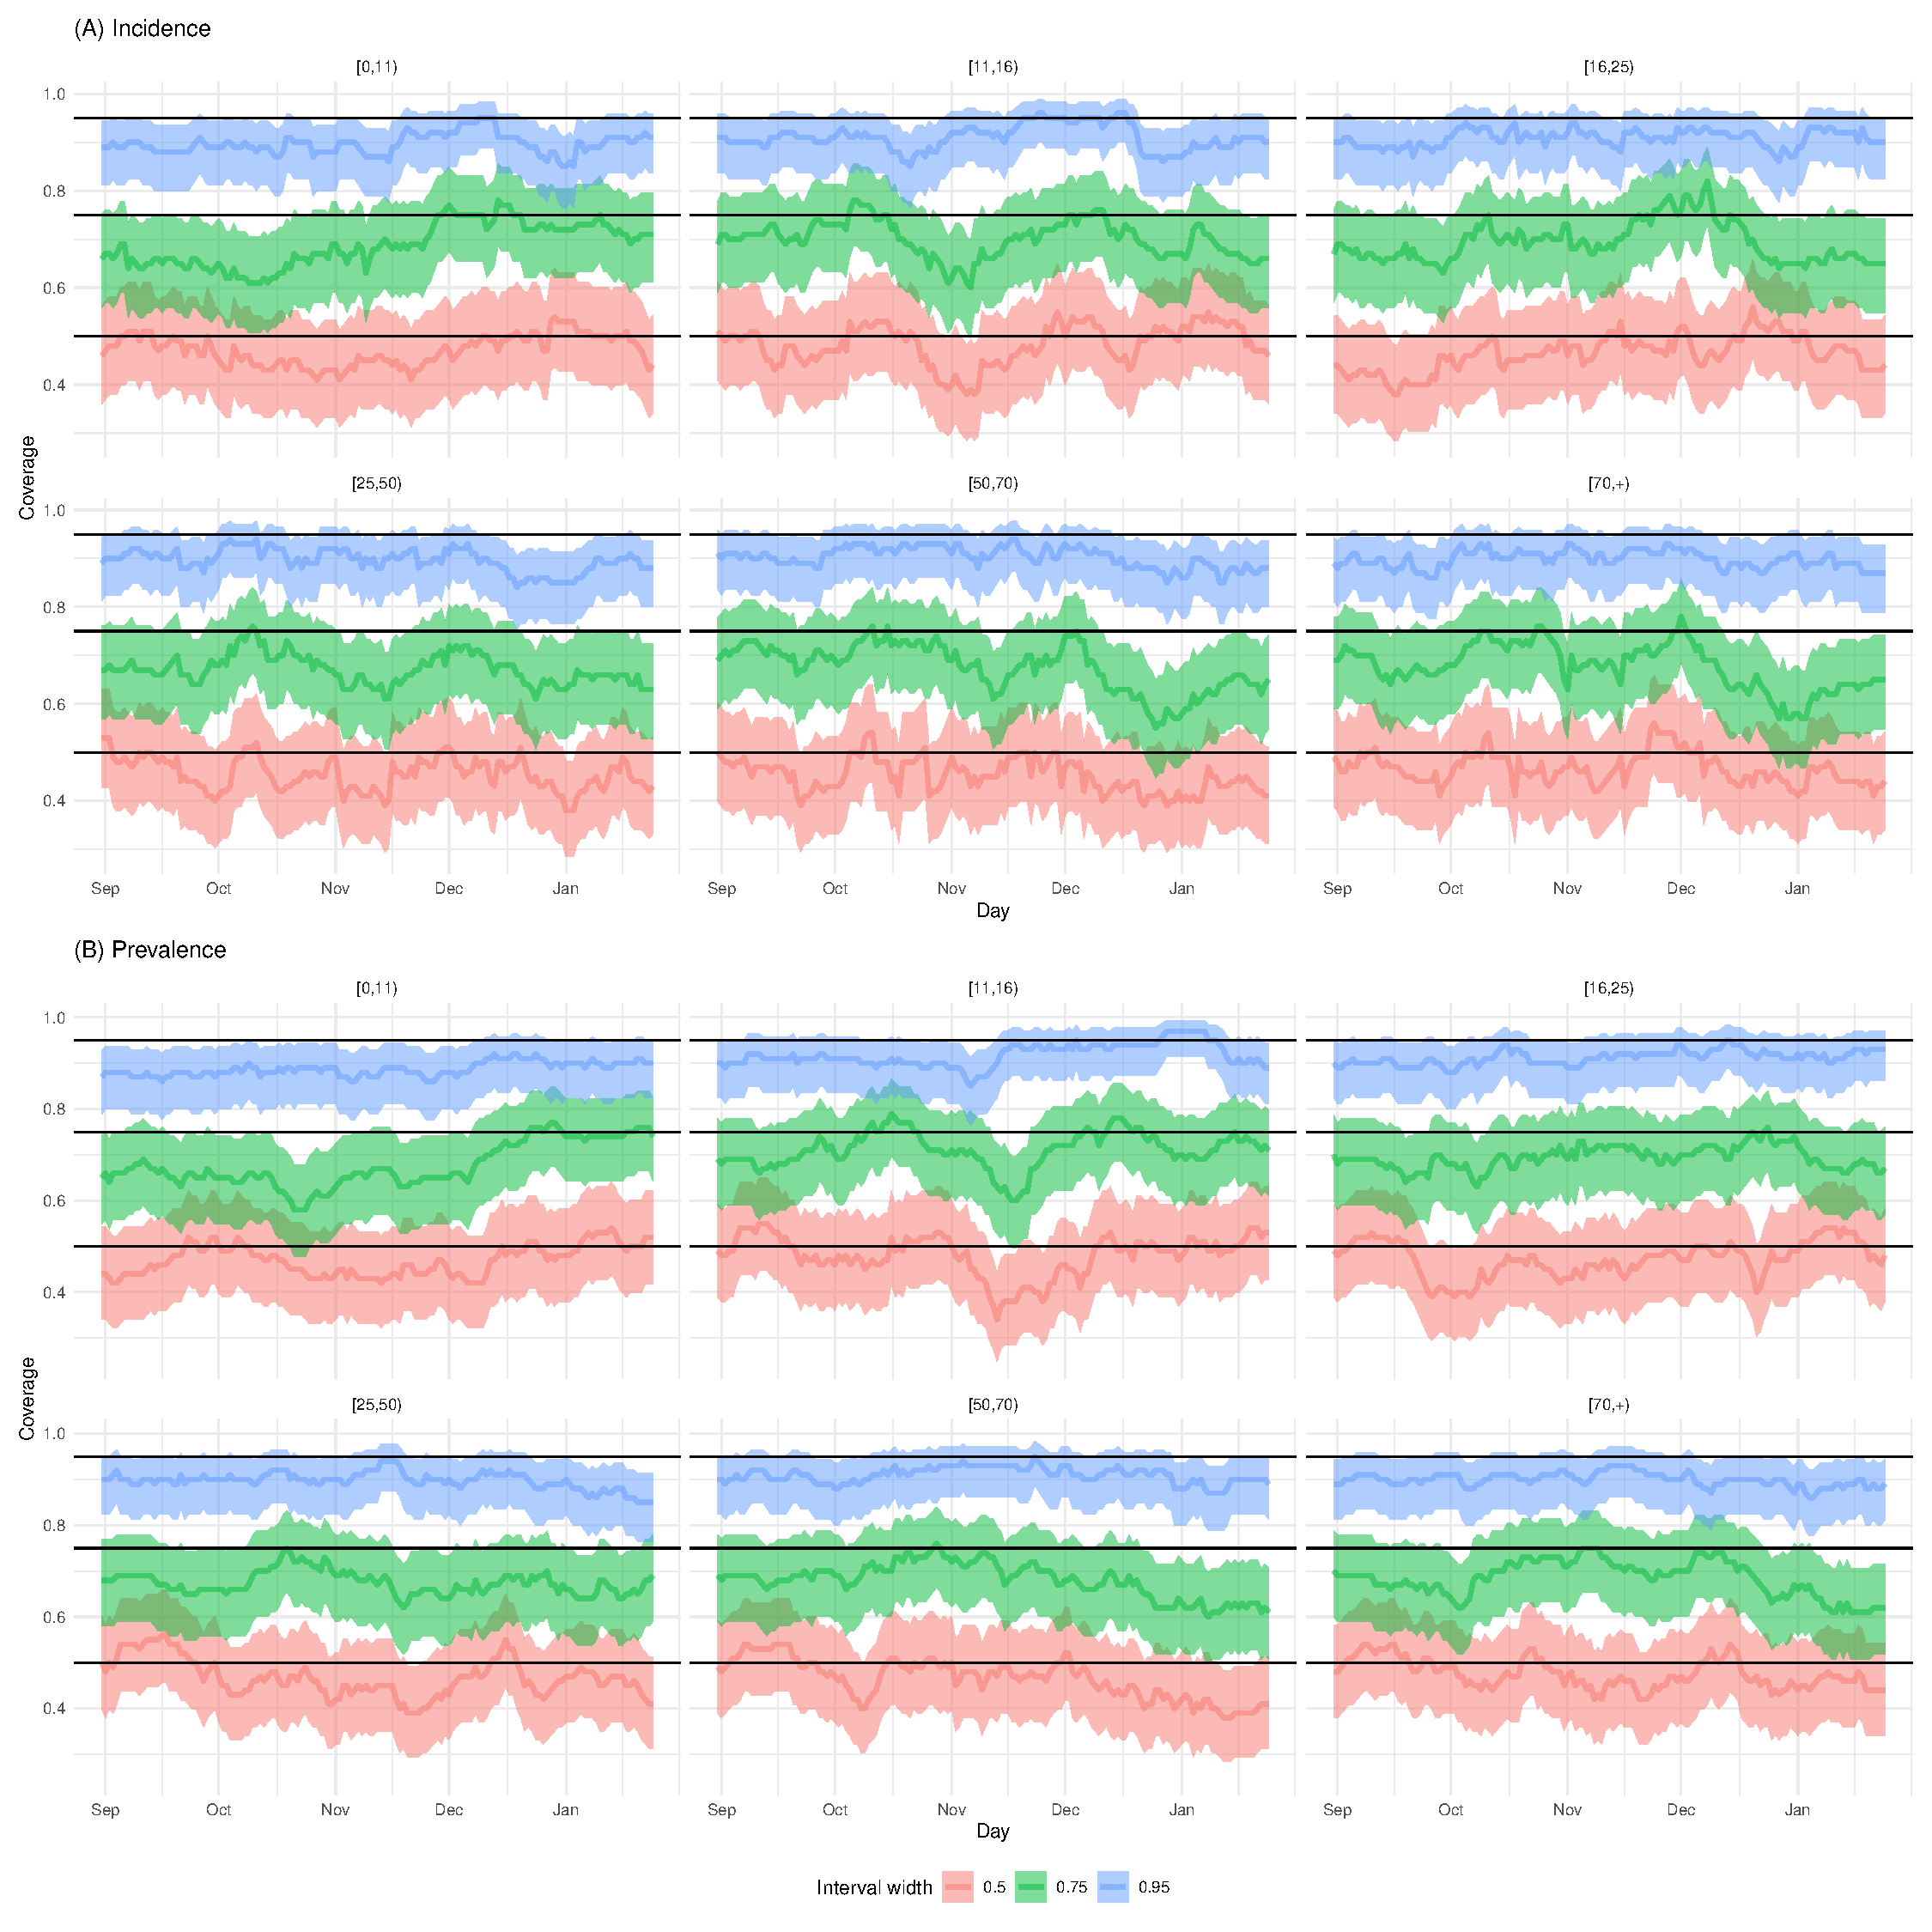
\includegraphics[width=0.9\paperwidth]{SEIR/sim/predictive_coverage}}
    \caption[Coverage of simulation study (derived quantities)]{%
        Point estimate and 95\% confidence interval for coverage of the 50\%, 75\%, and 95\% central credible intervals for incidence (top) and prevalence (bottom); see text for full definition.
        Horizontal lines show the nominal coverage.
    }
    \label{SEIR:fig:sim-inc-prev}
\end{figure}


In this setup, the parameters $i^+$, $q_c$, and $\psi$ are fully recovered; the other parameters are only partially so: their posterior has moved away from the prior but is still regularised by it (see \cref{SEIR:fig:true-vs-posterior}).
The ability to identify $q_c$ is an advantage of using data which includes measurements on children, unlike data on hospitalisations or deaths.

For $\vec{\pi}$ and $\rho$, the posterior median is very similar regardless of the true value (see \cref{SEIR:fig:true-vs-posterior}).
This suggests that these parameters are not practically identifiable in this setting.
The posteriors align very closely with the priors (not shown) which reinforces this finding.
The lack of identifiability for $\vec{\pi}$ aligns with previous work showing this parameter is structurally unidentifiable, \ie not identifiable even in the limit of infinite data~\autocite{dankwaStructural}.
\begin{figure}
    \makebox[\textwidth][c]{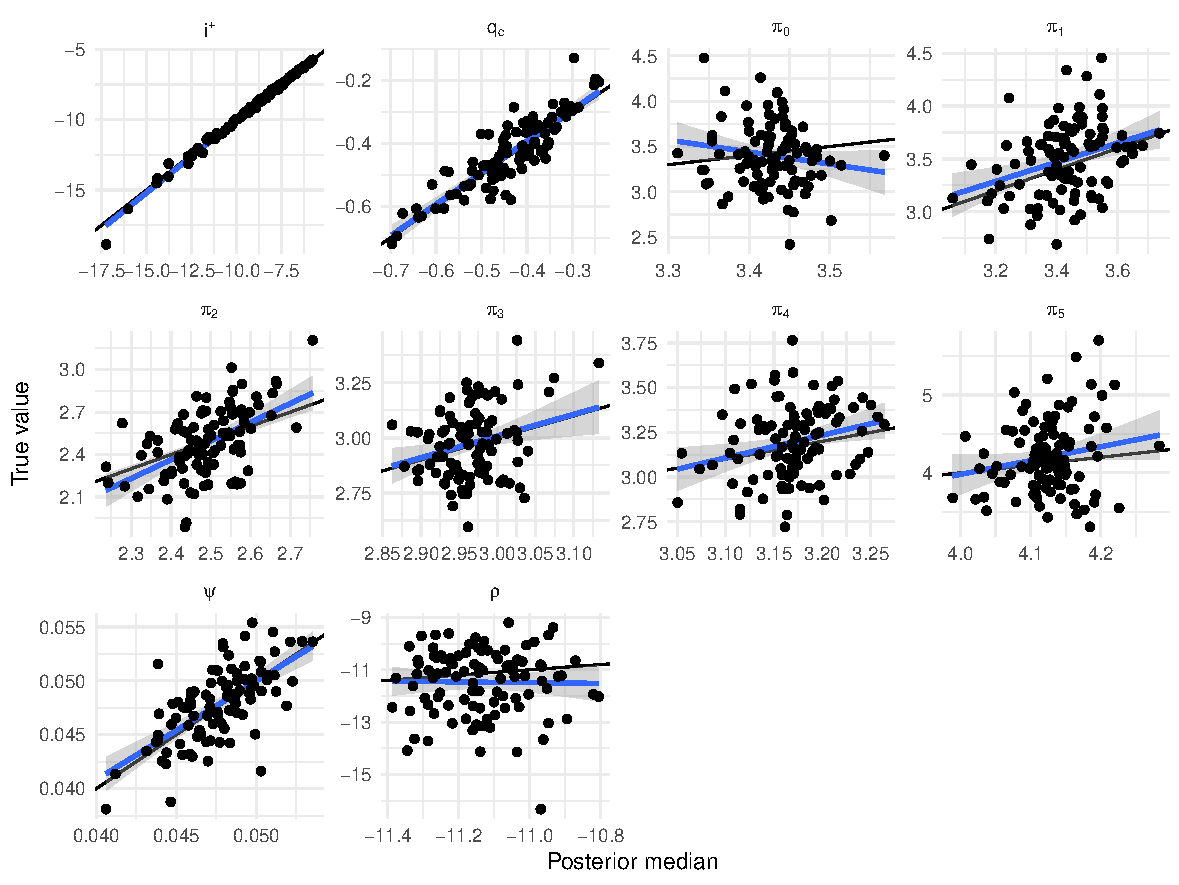
\includegraphics{SEIR/sim/true_vs_posterior}}
    \caption[True vs posterior parameter values]{%
        True vs posterior median parameter values for each parameter in each simulation.
        The black line shows the line $y = x$ which the dots would lie on if the parameter is fully recovered.
        The blue line is a linear regression line.
        For $i^+$, $q_c$, and $\psi$, the posterior recovers the true values.
        For $\vec{\pi}$ and $\rho$, the posterior median is very similar regardless of the true value.
    }
    \label{SEIR:fig:true-vs-posterior}
\end{figure}

\subsection{Application to CIS data} \label{SEIR:sec:application}

The 11--16 age group (roughly corresponding to compulsory secondary school education) is estimated to have the highest incidence (see \cref{SEIR:fig:incidence}).
Incidence is smooth within each week but shows discontinuities between weeks.
This is because the parameters within $\matr{\beta}(t)$ are constant within each week.
A constant $\matr{\beta}(t)$ would lead to exponential growth following a period of transitory dynamics, although the weekly switching may mean that these transitory dynamics never end, especially when incidence is high~\autocite{rhodesConvergence}.
When the peak in incidence is estimated to occur varied by region, with the most common time being early January 2021 (see \cref{SEIR:fig:peak-incidence}).
\begin{figure}
    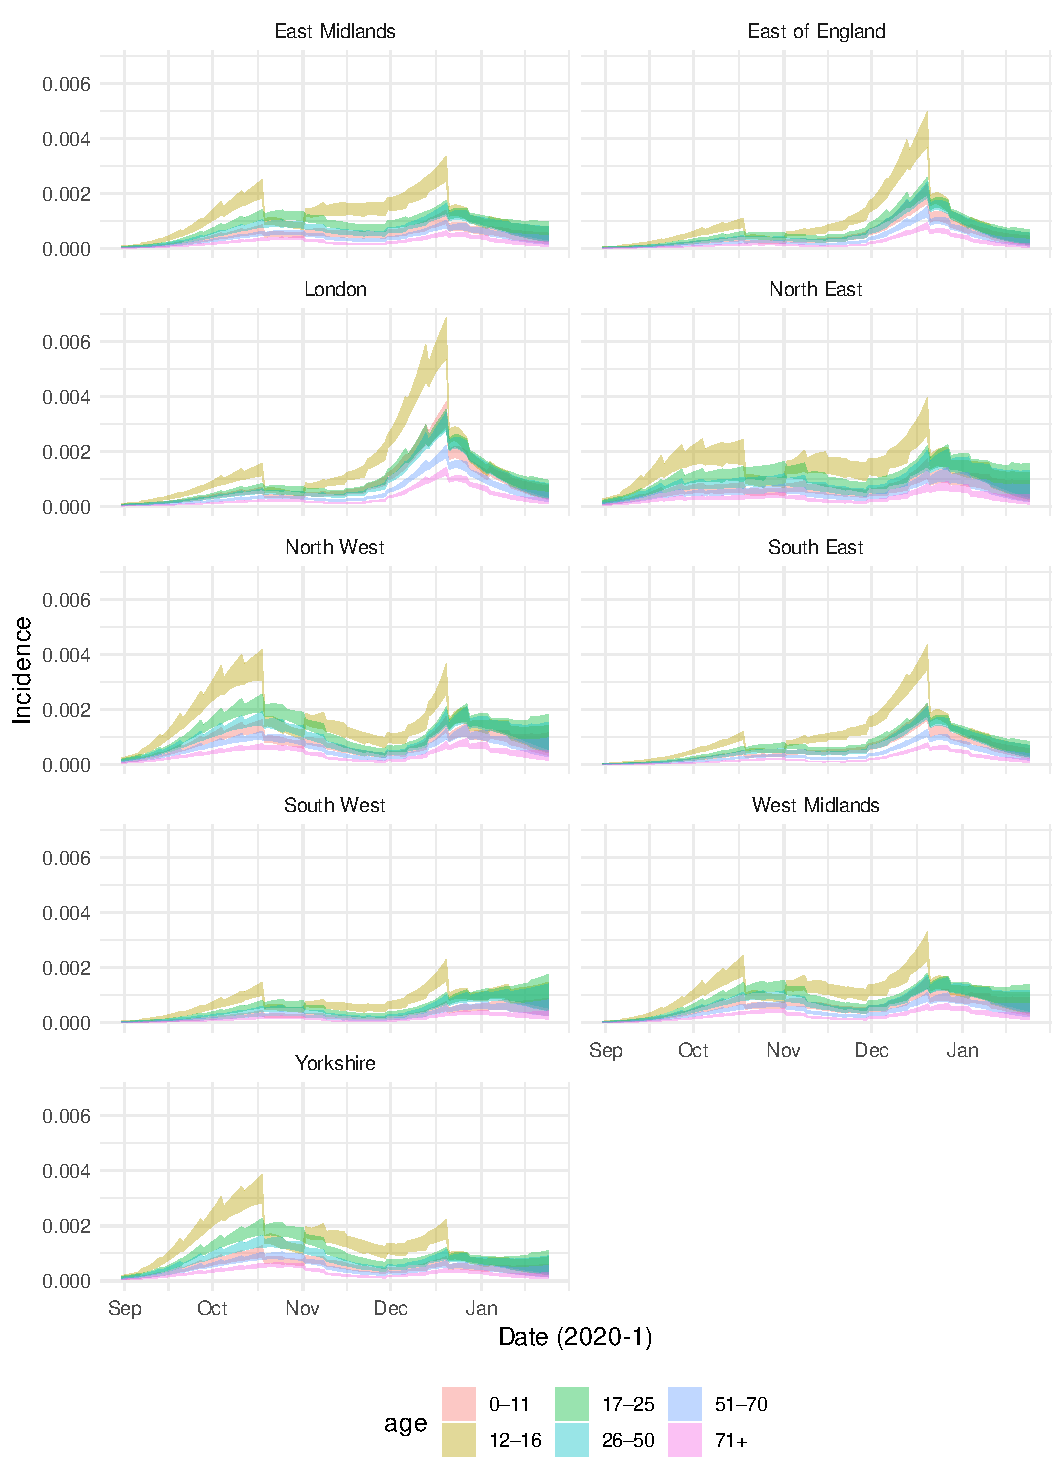
\includegraphics{SEIR/CIS/incidence}
    \caption[Posterior estimates of incidence]{%
        Posterior estimates (95\% CrI) of incidence by region and age.
        See main text for discussion.
    }
    \label{SEIR:fig:incidence}
\end{figure}
\begin{figure}
    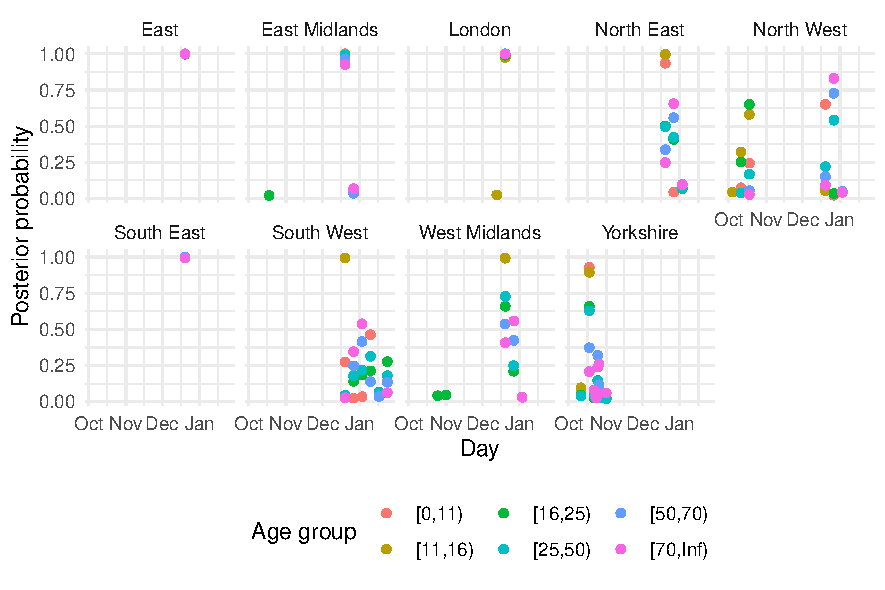
\includegraphics{SEIR/CIS/p_peak}
    \caption[Posterior estimates of peak incidence timing]{%
        Posterior probability of the peak incidence for each region and age combination occurring on each day.
    }
    \label{SEIR:fig:peak-incidence}
\end{figure}

The $\beta_w$ parameters absorb all the time-varying changes in transmission not captured by Google mobility and school attendance data.
They trend downwards up until early December, then they start increasing (see \cref{SEIR:fig:beta-walk}).
Correlation is clear across the regions even though each region is estimated independently, suggesting underlying biological or epidemiological changes across regions as opposed to modelling assumptions.

\begin{figure}
    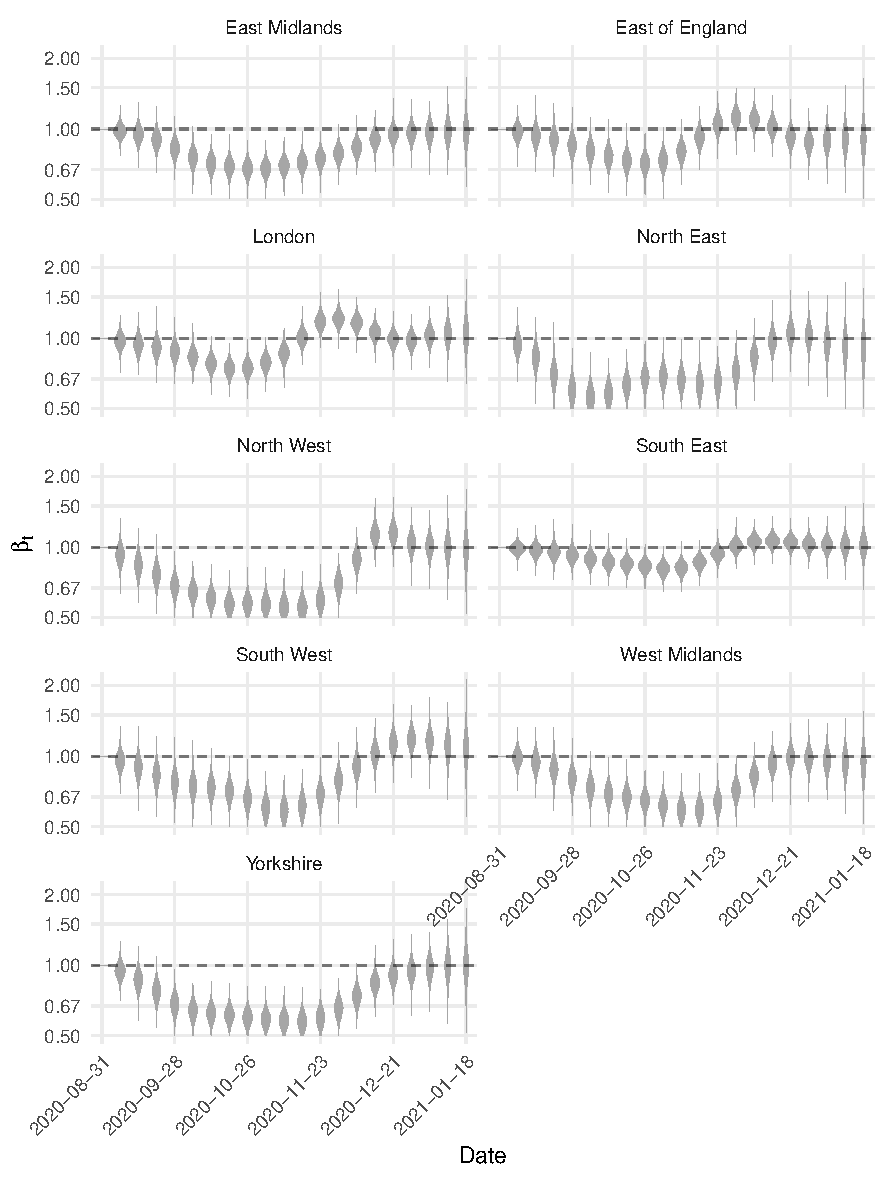
\includegraphics{SEIR/CIS/beta_walk}
    \caption[Posterior estimates of $\beta_w$]{%
        Posterior estimates $\beta_w$ for each week.
        Shown are ``violins'' where the width is proportional to the kernel-density estimated posterior density at that point.
        Values trend downwards until early December when an increase starts.
    }
    \label{SEIR:fig:beta-walk}
\end{figure}

The \emph{attack rate} is the proportion of the population that have been infected at least once\todo{cite attack rate}.
In this model it is $1 - \vec{s}$, the proportion susceptible.
The attack rate is highest in the $[11, 16)$ age group in the North West at 68\% (95\% CrI: 66\%--70\%) (see \cref{SEIR:fig:attack-rates}).
\begin{figure}
    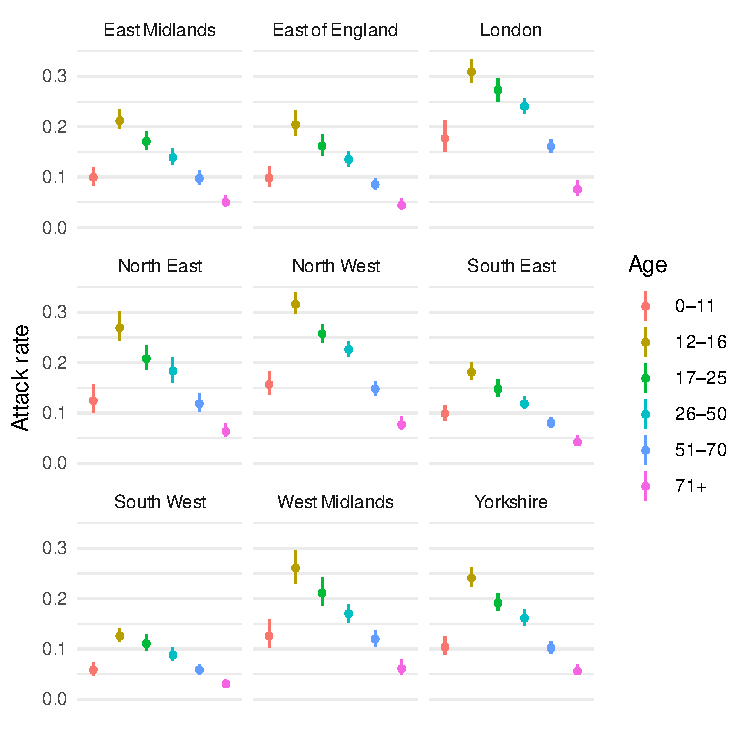
\includegraphics{SEIR/CIS/attack_rates}
    \caption{Posterior median and 95\% CrI of the attack rate in each region and age group.}
    \todo[inline]{Maybe compare this to blood donors, as used in the prior.}
    \label{SEIR:fig:attack-rates}
\end{figure}

Overall the model fits the data well (see \cref{SEIR:fig:prev-young,SEIR:fig:prev-old}).
There are a few features of the data which are not captured by the model and the posterior estimate appears to be a compromise with the prevalence too low in one age group and too high in another.
For example, in the North East region, the 11--16 age group has its prevalence overestimated in October but the 16--25 age group has its prevalence underestimated.
\begin{figure}
    \thisfloatpagestyle{empty}
    \vspace{-3cm}
    \makebox[\textwidth][c]{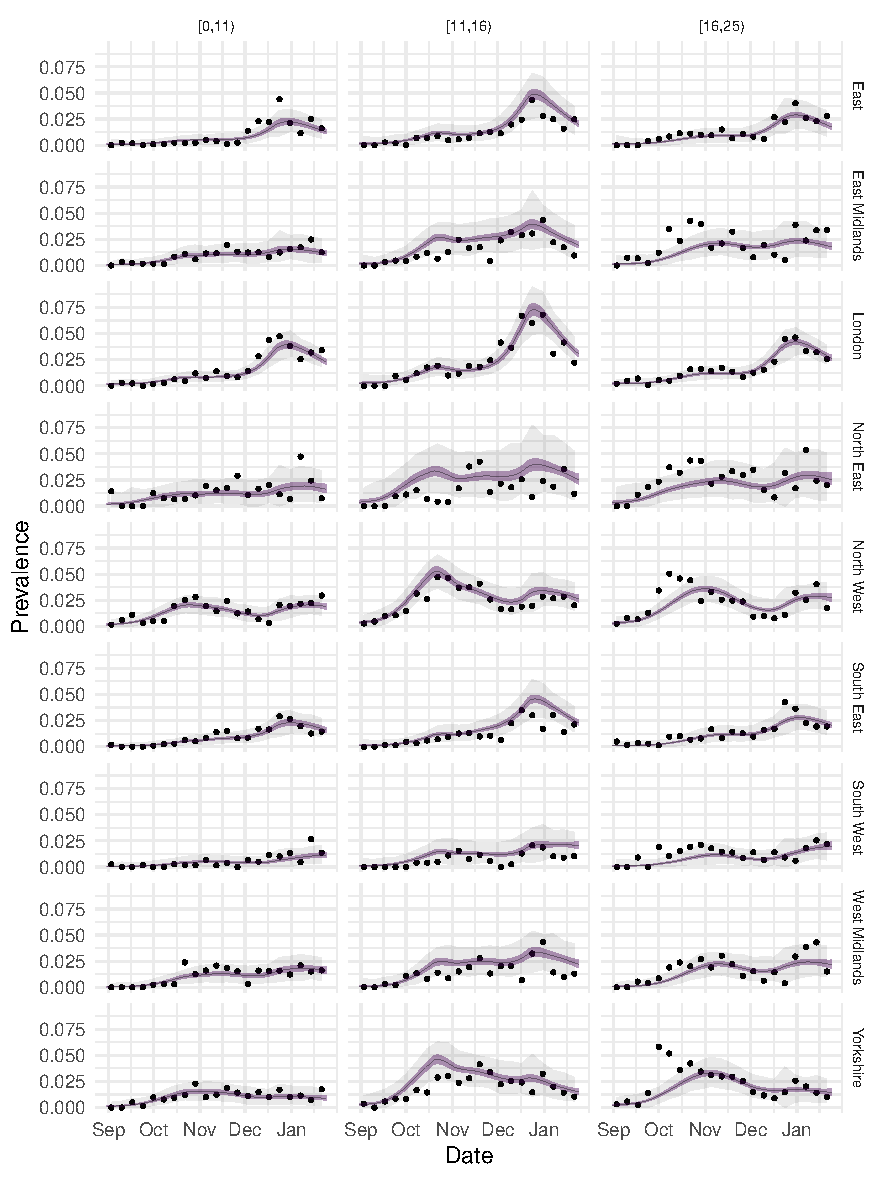
\includegraphics[width=.9\paperwidth]{SEIR/CIS/prev_young}}
    \captionsetup{width=0.8\paperwidth}
    \captionof{figure}[SEIR prevalence goodness-of-fit (younger ages)]{%
        Goodness-of-fit to prevalence data by region and age for the younger three age groups (see \cref{SEIR:fig:prev-old} for the others).
        The central ribbon and line shows the posterior median and 95\% CrI estimate for the proportion of the relevant strata RT-PCR positive on each day.
        The lighter outer ribbon is the 95\% posterior predictive interval for the proportion of test results that are positive each week.
        The dots show the observed prevalence in CIS, aggregated by week.
        For a well-calibrated model, 95\% of the dots would be within the outer ribbon.
    }
    \label{SEIR:fig:prev-young}
\end{figure}
\begin{figure}
    \thisfloatpagestyle{empty}
    \vspace{-3cm}
    \makebox[\textwidth][c]{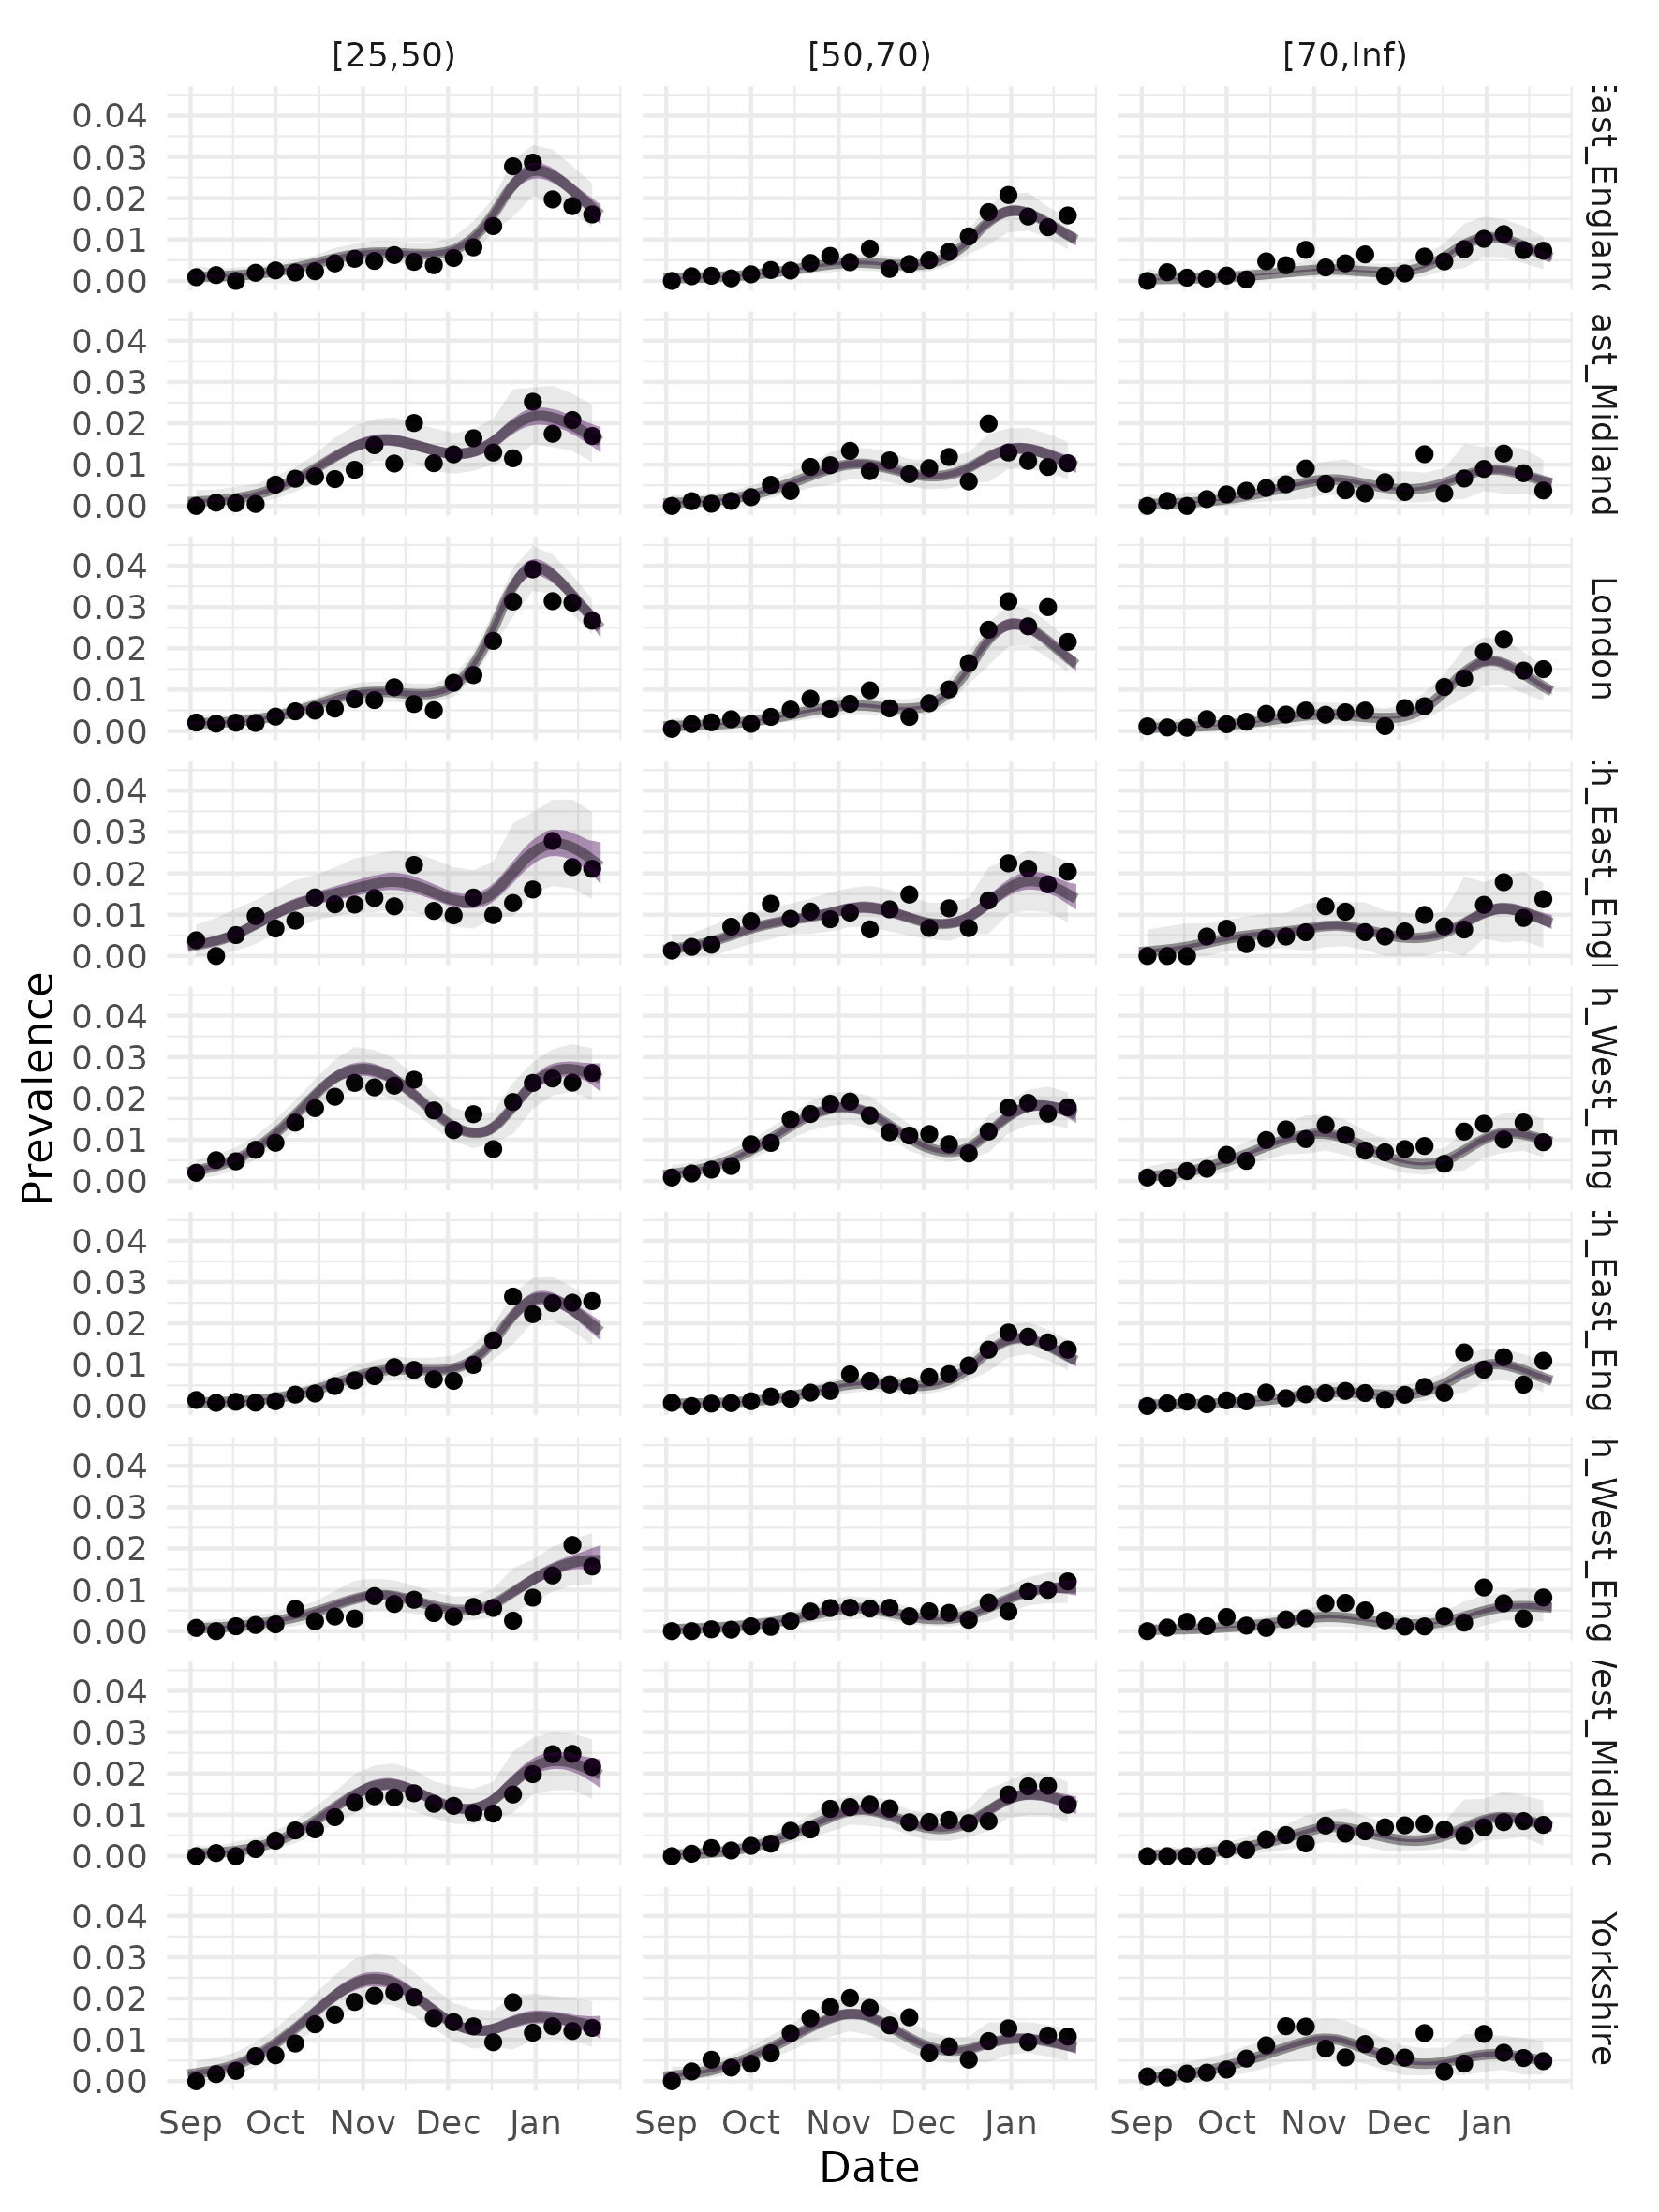
\includegraphics[width=.9\paperwidth]{SEIR/CIS/prev_old}}
    \captionsetup{width=0.8\paperwidth}
    \captionof{figure}[SEIR prevalence goodness-of-fit (older ages)]{%
        Goodness-of-fit prevalence for the older three age groups (see \cref{SEIR:fig:prev-young} for the other age groups and details).
    }
    \label{SEIR:fig:prev-old}
\end{figure}

All regions' MCMC chains converged, assessed using the Rhat statistic and ESS (as defined in \cref{E-inc-prev:sec:MCMC}).
The lowest Rhat was 1.01 for $\sigma_\epsilon$ in London.
All parameters had ESS > 1000, except $\sigma_\epsilon$ and $\psi$ in London, which had ESS of 450 and 950 respectively.

\subsection{Discussion} \label{SEIR:sec:discussion}

The results in this section show the feasibility of fitting a mechanistic model using only data on prevalence.
If the distributions for length-of-stay in each compartment are known, then all other model parameters can  be estimated.
This includes the age distribution of the infections and the components of transmission.

% Unlike most prior work (see\todo{ref section with lit review}), this modelling is based on a data source that is representative of the general population.
% % Therefore, the results have fewer biases and informed by data to a greater extent than this work.
% There is little-to-no ascertainment bias in the CIS, unlike sources relying on testing behaviour (in the UK, pillar 2 testing).
% The CIS allows estimates of transmission in children, unlike sources relying on severe events that occur almost entirely in adults~\autocite{bhopalChildren}.
Using a mechanistic model provides additional understanding, compared to the approach in \cref{E-backcalc}.
For example, decomposing the change in transmission into changing contacts, $\matr{\kappa}(t)$, changing susceptibility $\vec{s}(t)$, and other unmeasured factors, $\beta(t)$.
By understanding which of these components is changing, policies can be better targeted.
If it is shown that $\beta(t)$ decreases, this implies that for a given contact rate in the population, there is less transmission.
Such decreases might be beneficial as it allows society to operate in a more normal manner without increasing transmission.
% Increasing activity without increasing transmission is desirable because it enables reductions the disease burden without burdesome restrictions on individuals day-to-day lives.


The parameters $\beta_w$ absorb all the time-varying factors not captured by Google mobility and school attendance data.
Many factors contribute to the pattern in the $\beta_w$ values, which have a minima near the start of December.
While this analysis cannot establish causation, several hypotheses that are worth considering.

The decreases in $\beta_w$ over the autumn could be due to increased caution (\eg masking or stricter adherence to social distancing) as cases and deaths increased~\autocite{jarvisEffect} and/or not captured by $\matr{\kappa}(t)$, such as the impact of local measures in the highest transmission areas~\autocite{scottCovid19}.
Local measures are not well captured by $\matr{\kappa}(t)$ because the matrix averages behaviour across the whole of England.
Allowing each region to have its own $\matr{\kappa}(t)$ may capture the effect of local measures more accurately, although their targeted nature may require more granular methods.

The increases in $\beta_w$ in December coincide with the rise of the Alpha variant~\autocite{lythgoeLineage}, known to be more transmissible~\autocite[e.g.][]{daviesEstimated}.
A multiple variant model might be able to capture this rise more accurately.
Such a model would stratify positive tests in the CIS by pre-Alpha or Alpha variant.
Then, each variant would be explicitly included in the model to fit to this data.

These hypotheses for the mechanism causing changes in $\beta_w$ are correlated across the country.
This can explain that similar patterns emerge for $\beta_w$ in different regions (see \cref{SEIR:fig:beta-walk}), despite these being estimated independently (\ie there is no model structure which favours correlated values).
These correlations could be exploited to improve the precision of estimates with a more complex model which borrows information across regions.

The current model could be more flexible with regards to the age distribution of infections.
This would better exploit one of the strengths of the CIS: the availability of data  on all age groups.
In some regions, there appears to be a trade-off between the 11--16s and 16--25s, with the model misfitting in opposite directions (see \cref{SEIR:fig:prev-young}).
This implies that the data would allow identification of a more flexible age-based model.

Currently, the age distribution of infections is determined by $\matr{\beta}$, and to a lesser extent $\vec{\pi}$, the former of which only contains one parameter that affects the age distribution, $q_c$.
Increasing the number of parameters in $\matr{\beta}$ would be the simplest approach to increase the model's flexibility.

The only time-changing part of $\matr{\beta}$ that varies between ages is $\matr{\kappa}$.
It is plausible that this would not capture all behavioural changes.
For example, the introduction and relaxation of control measures within schools.
$\matr{\kappa}$ only captures changes in in-school transmission through changes in school attendance, not incorporating the probability of transmission, which could be modelled as changes in $q_{aa}$ for $a$ of school age.
Similarly, there is evidence that $q_c$ is different for Alpha and pre-Alpha variants~\autocite{zhuRole}, which could again motivate these changing over time.

The weekly patterns in incidence are a limitation of the current parameterisation.
The random walk and contact matrices both vary only on the weekly timescale.
A daily random walk could provide more flexibility here.
However, this would greatly increase the number of parameters.
An alternative would be a smoothly-varying function or an approximation of a random walk, such as that proposed by \textcite{ghoshApproximate}.

This discussion makes clear that the results are limited by the number of parameters, currently limited by the inference algorithm.
\todo{Rephrase this sentence}
The algorithm used here tends to struggle with a large number of parameters.
Alternative proposal schemes, such as updating the parameters in blocks\todo{cite what RTM does?}, could help, or a more advanced algorithm such as NUTS (used elsewhere in this thesis).

Extending the analyses carried out here to the rest of the pandemic would clearly be of interest.
I chose the end of the period to coincide with the vaccination rollout.
Vaccination dramatically affects the transmission dynamics by introducing some additional immunity into the population.
Mechanistic models require explicit representation of this immunity\todo{cite something about vaccination, including new RTM paper}.

\section{Comparison of results} \label{transmission:sec:comparison}

\Cref{transmission:fig:compare-regions} compares the regional incidence estimates between the two models in this chapter.
Generally the estimates agree, with the SEIR model having much narrower credible intervals.
The largest discrepancy is that the backcalculation model estimates a second peak in mid January in several regions (most clearly in London, North West, and the East of England).
However, except in London, the credible intervals still overlap.
This is a specific case of a larger pattern: the SEIR model produces smoother estimates of incidence than the backcalculation model.;
\begin{figure}
    \centering 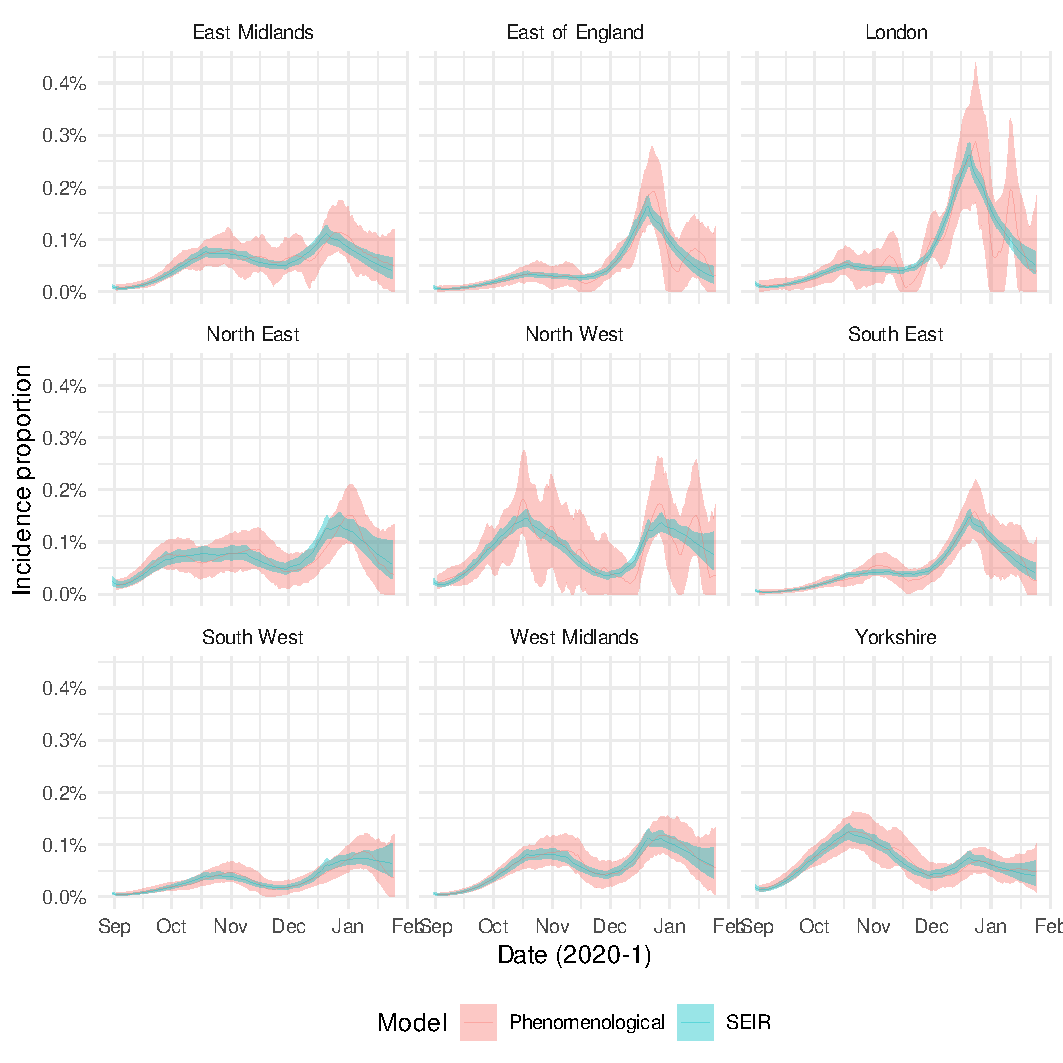
\includegraphics{transmission/compare-regions}
    \caption[Comparing each models estimate of regional incidence.]{%
        Incidence proportion in England and each region estimated by the two models discussed in this chapter.
        Posterior median and 95\% CrI shown.
        For the SEIR model, newly RT-PCR positive (entrances into the P1 compartment), rather than incidence (entrances into the E compartment) are shown for comparability with the backcalculation results.
    }
    \label{transmission:fig:compare-regions}
\end{figure}

These patterns can be interpreted as an instance of the common bias---variance trade-off.
The SEIR model imposes stronger assumptions about the epidemic dynamics.
The assumptions reduces the variance of the estimates, including by making them smoother, but if the assumptions are incorrect, bias is introduced.
This trade-off based on the strength of assumptions has long been known to apply in the backcalulcation context~\autocite[e.g.][section 8.3]{brookmeyerBackcalculation}.
The SEIR model can be viewed as a backcalulation method where the transmisson part of the model is a smoothing method.

The backcalculation method benefits from being able to be implemented in a fast, approximate inference package (R-INLA) that easily scales to many parameters, including random effects.
Therefore, it is far more flexible and can easily include time-varying effects, ethnicity, etc.
The SEIR model is limited by the inference procedure and the requirement to sovle an ODE to evaluate the likelihood.
To incorporate a more flexible model, and reduce its bias, a more efficient inference procedure would be required.

Many of these issues are clearly demonstrated by the estimates for the North East (see \cref{transmission:fig:compare-NE}).
I previously observed the quality of the SEIR model's fit is variable between different age groups (see \cref{SEIR:fig:prev-young,SEIR:fig:prev-old}).
This is because the model is not flexible enough to capture the true age distribution of infections.
The overestimation of prevalence in the 11--16 age group and underestimation in the 16--25 age group is reflected when comparing incidence estimates to those from the backcalculation model, which have reduced bias.
\begin{figure}
    \centering 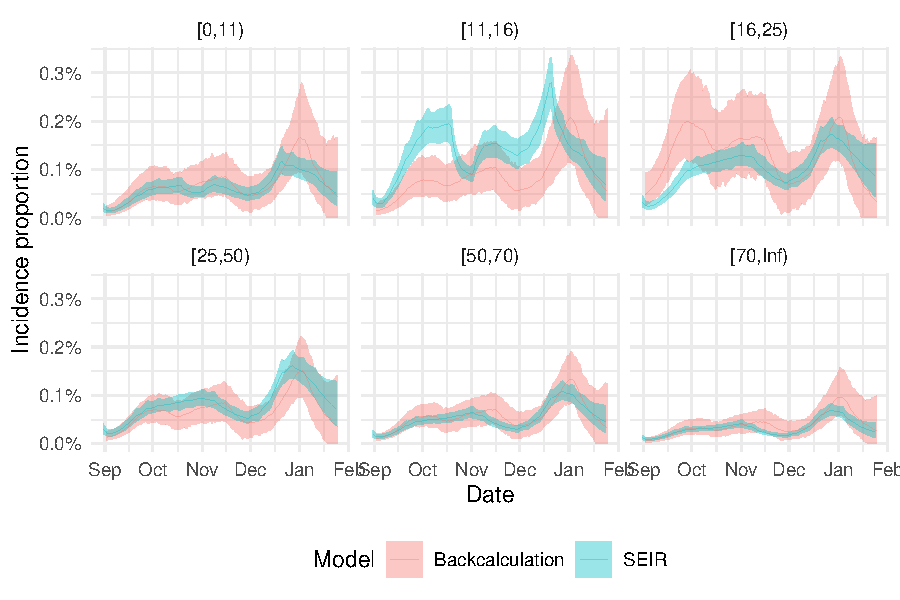
\includegraphics{transmission/compare-NE}
    \caption[Comparing each models estimate of North East incidence by age.]{%
        Incidence proportion in each age group in the North East estimated by the two models discussed in this chapter.
        Posterior median and 95\% CrI shown.
        For the SEIR model, newly RT-PCR positive (entrances into the P1 compartment), rather than incidence (entrances into the E compartment) are shown for comparability with the backcalculation results.
    }
    \label{transmission:fig:compare-NE}
\end{figure}


\section{Conclusion}

The major contribution in this chapter is showing that transmission and incidence can be estimated using only data from the CIS.
A similar survey could, therefore, be considered as the primary form of surveillance for a future pandemic.
The advantage of such a setup is the unbiased information across the entire population, including children.

The transmission model presented in this chapter could be extended to fully extract the information in the CIS (see \cref{SEIR:sec:discussion}).
This would require a more flexible model, which would likely require a more efficient inference procedure, such as NUTS.



\ifSubfilesClassLoaded{
  \listoftodos
}{}

\end{document}